\documentclass[utf8]{gradu3}

\usepackage[utf8]{inputenc}
\usepackage{graphicx} % kuvien mukaan ottamista varten
\usepackage{amsmath} % hyödyllinen jos tekstisi sisältää matikkaa,
                     % ei pakollinen
\usepackage{booktabs} % hyvä kauniiden taulukoiden tekemiseen
\usepackage{comment}
\usepackage{tikz}

\usepackage{tabularx}
\usepackage{ragged2e}
\usepackage{adjustbox}
\usepackage{lipsum}

% HUOM! Tämän tulee olla viimeinen \usepackage koko dokumentissa!
\usepackage[bookmarksopen,bookmarksnumbered,linktocpage]{hyperref}

\addbibresource{gradulahteet.bib} % Lähdetietokannan tiedostonimi


\begin{document}

\title{Systemaattinen kirjallisuuskatsaus perehdyttämiskäytännöistä ohjelmistokehitysorganisaatioissa (v. 0.3.0)}


\translatedtitle{TODO}
\studyline{Ohjelmisto- ja tietoliikennetekniikan opintosuunta}
\avainsanat{TODO}
\keywords{TODO}

\tiivistelma{TODO}
\abstract{TODO}

\author{Jessica Sarlin}
\contactinformation{\texttt{jessica.sarlin@gmail.com}}

\supervisor{Antti-Jussi Lakanen}

\maketitle

\mainmatter

\chapter{Johdanto}

% Miksi työ ohjelmistoalalla on haastavaa? (asiakkaiden lukuisat toiveet, rajallinen käytettävissä oleva aika, haastavaa rakentaa ohjelmistoja, jotka on helppo käyttää, ylläpitää ja laajentaa, yksittäiseen työtehtävään kuluvaa aikaa vaikea arvioida etukäteen)

% Kun maailma digitalisoituu ja kaikkialla on koodia, tarvitaan jatkuvasti vahvempaa ja parempaa osaamista. Ihan ok ei riitä, jos ja kun maailma ja kaikki yhteiskunnan kriittiset asiat pyörii koodilla!

Hyvä perehdytys työsuhteen alkaessa on tärkeää sekä työntekijöille että työnantajille. Huolellisella perehdytyksellä voidaan varmistaa, että uudet työntekijät saavat työssään tarvitsemansa tiedot ja taidot. Se on tärkeä osa työntekijöiden integroitumista työyhteisöön ja auttaa heitä omaksumaan työkulttuuriin ja -käytäntöihin liittyviä asioita. Hyvä perehdytys on tärkeää heidän onnistumiselleen, sitoutumiselleen ja tyytyväisyydelleen työssään, ja sen avulla voidaan myös vähentää virheitä ja parantaa työskentelytehokkuutta. Erityisen tärkeää perehdytys on työuran alussa.

Ohjelmistokehityksen alalla on paljon tarvetta kokeneille osaajille eli senioreille. Jokainen alalle tulija kuitenkin aloittaa juniorina, josta vähitellen kehitytään kokeneeksi osaajaksi - esimerkiksi \textcite{bologa-lupu-2014} tämä voivan kestää jopa kaksi vuotta. Ohjelmistokehitystyön luonne abstraktina ongelmanratkaisuna tuo omat haasteensa perehdyttämiselle. On tärkeää, että yksilöiden osaaminen kehittyy, jotta alalla on jatkossakin osaavia asiantuntijoita.

Tämän tutkimuksen tavoitteena on selvittää ohjelmistokehitysorganisaatioiden käyttämiä perehdyttämiskäytäntöjä ja luoda niistä synteesiä, jotta niitä voitaisiin helpommin hyödyntää. Tutkimusmenetelmänä on systemaattinen kirjallisuuskatsaus.

\textbf{TODO lisää akateeminen motivaatio}

\textbf{TODO kerrottava miksi tehtiin, ja sekä akateemista että käytännön merkitystä}

\chapter{Teoriaosa}

Tässä luvussa eritellään perehtymisen käsitettä, sen tärkeyttä ja hyötyjä sekä työuran alun erityisyyttä ohjelmistoalalla.

\textbf{Ohjaajan kommentti 3.1.2023: "Omasta mielestäni järjestys voisi mennä niin, että keskustelet ensin auki haasteen nimen omaan liittyen ohjelmistoalaan. Nyt se on vasta luvussa 2.5. Mielestäni tätä motivaatiota vasten olisi sitten luonteva esittää noita teorioita, viitekehyksiä ja aikaisempia tutkimustuloksia."}

\section{Organisatorisesta sosialisaatiosta perehdyttämiseen}
Jotta perehdyttämistä voidaan ymmärtää, hahmottaa ja tutkia, on aluksi tarpeen käsitellä sitä, miten perehdyttämisen käsitettä on kirjallisuudessa pyritty määrittelemään.

\textcite{wanberg-2012} toteaa, että perehdyttämisen yläkäsite on organisatorinen sosialisaatio (eng. \textit{organizational socialization}). Sillä \textcite{wanberg-2012} tarkoittaa organisaatioon hiljattain liittyneessä ihmisessä tapahtuvaa prosessia, jossa hän hankkii uuteen työtehtävään sopeutumiseen tarvittavat tiedot, taidot, asenteet ja toimintatavat. Myös \textcite{chao-2012} toteaa, että organisatorinen sosiaalistuminen on oppimis- ja sopeutumisprosessi, jonka avulla yksilö voi omaksua roolin, joka vastaa sekä organisaation että yksilön itsensä tarpeita. \textcite{chao-2012} toteaa organisatorisen sosialisaation käsitteen kattavan sekä organisaation että yksilön pyrkimykset työhön sopeutumiseen.

\textcite{saks-gruman-2012} taas määrittelevät organisatorisen sosialisaation käytännöiksi nimenomaan organisaation aloitteesta tapahtuvat ohjelmat, tapahtumat ja kokonaisuudet, joiden tavoitteena on helpottaa uusien tulokkaiden oppimista ja sopeutumista työhön, työryhmään ja rooliin, varmistaen näin että tulokkaista tulee organisaation tehokkaita jäseniä. \textcite{saks-gruman-2012} tekevät vielä erikseen eron organisaation aloitteesta tapahtuviin toimiin, erottaen ne työntekijän itsensä aloitteesta tehtäviin.

\textcite{wanberg-2012} toteaa, että perehdyttäminen taas on organisatorista sosiaalistumista kapeampi käsite. Hänen mukaansa sosiaalistumisen prosessi voi toki sisältää perehdyttämistä, mutta se kattaa myös laajempia tiedonhaun, oppimisen ja sopeutumisen osaprosesseja. Myös \textcite{klein-polin-2012} korostavat, että sosialisaatio on prosessi, joka tapahtuu yksilön sisällä. He toteavat, että perehdyttämisellä tarkoitetaan niin muodollisia kuin epämuodollisiakin käytäntöjä, toimintatapoja ja toimia, joita organisaatio tai sen edustajat käyttävät helpottaakseen uusien tulokkaiden sopeutumista.

%\textcite{chao-2012} toteaa, että organisatorisen sosialisaation käsitettä on käytetty perehdyttämisen rinnalla. Hän kuitenkin toteaa, että perehdyttämisen käsitettä näytetään käytettävän vain uusien työntekijöiden kohdalla eli ei silloin, kuin työntekijä vaihtaa tehtäviä organisaation sisällä. 

\textcite{klein-polin-2012} määrittelevät perehdyttämiseksi joukon käytäntöjä, toimintatapoja ja menettelyjä, joita esihenkilöt ja HR-osastot käyttävät jäsentääkseen uusien työntekijöiden ensimmäisiä kokemuksia ja helpottaakseen siten uusien työntekijöiden sosiaalistumista.

Myös tässä tutkimuksessa perehdyttämisen käsite ymmärretään nimenomaan organisaation aloitteesta tapahtuvaksi toiminnaksi. Uuden työntekijän oma toiminta vaikuttaa toki organisatoriseen sosiaalistumiseen, mutta tässä tutkimuksessa tarkastelun kohteena ovat nimenomaan organisaatiosta lähtevät käytännöt.

\section{Perehdyttämisen hyödyt}

Miksi uusien työntekijöiden perehdyttäminen sitten on tärkeää? \textcite{saks-gruman-2012} toteavat, että uudessa työpaikassa aloittavat työntekijät kokevat usein epävarmuuden ja vierauden tunteita liittyen omaan rooliinsa, suoriutumiskykyynsä ja organisaation toimintatapoihin. Uuden työn aloittamiseen ei siis liity ainoastaan työn itsensä suorittamiseen liittyvää epävarmuutta, vaan moniuloitteisia sosiaalisia ulottuvuuksia \parencite{saks-gruman-2012}. 

\textcite{wanberg-2012} toteaa, että onnistunut organisatorinen sosiaalisaatio voi johtaa lisääntyneeseen työntekijöiden tyytyväisyyteen, sitoutuneisuuteen, työssä pysymiseen ja hyvään suoriutumiseen. Myös \textcite{bauer-ym-2007} toteavat, että työntekijöiden sopeutumisen osatekijät (selkeä käsitys omasta roolista, vahva minäpystyvyys ja sosiaalinen hyväksyntä) olisi yhteydessä työssä koettuun tyytyväisyydeen, työhön sitoutumiseen, hyviin työsuorituksiin ja vähäiseen vaihtuvuuteen. 

\textcite{saks-gruman-2012} toteavat, että organitorisen sosialisaation tuloksia tarkasteltaessa voidaan tehdä ero lähitulosten (engl. \textit{distal outcomes}) ja kaukotulosten (eng. \textit{proximal outcomes}) välille. Lähituloksiin on myös viitattu uuden työntekijän sopeutumisena ja esimerkeiksi mainitaan työntekijän kokema roolien selkeys, oppiminen ja minäpystyvyys. Kaukotuloksilla taas tarkoitetaan perinteisempiä sosiaalistumisen tuloksia kuten työtyytyväisyyttä ja organisaatioon sitoutumista. Sosialisaatiokäytäntöjen hyödyntämisen katsotaan johtavan lähituloksiin, joiden puolestaan katsotaan johtavan kaukotuloksiin. \parencite{saks-gruman-2012}.

Vaikuttaa siis siltä, että uusien työntekijöiden perehdyttämiseen panostamalla voidaan edistää työntekijöiden organisatorisen sosialisaation onnistumista. Hyvä perehdytys varmistaa, että uudet tulokkaat saavuttavat työssään tarvittavat tiedot ja taidot sekä onnistuakseen tehtävissään että sitoutuakseen työpaikkaansa.

Miten perehdyttämisen käytännön toteutusta eli perehdyttämiskäytäntöjä sitten voidaan jäsentää? Kirjallisuudessa aihetta on lähestytty eri näkökulmista. \textcite{saks-gruman-2012} jäsentävät organisatorisen sosialisaation kirjallisuudessa esiteltyjä käytäntöjä jakaen ne viiteen ryhmään, minkä pohjalta he esittelevät oman sosialisaatioresurssien teoriansa. Seuraavissa luvuissa tutustutaan ensin näihin viiteen ryhmään ja kyseiseen teoriaan.

\section{Käytäntöjen jaottelua}

\textcite{saks-gruman-2012} siis jakavat organisatorisen sosialisaation käytännöt viiteen ryhmään: orientaatio-ohjelmat, työnopetusohjelmat, sosialisaatiotaktiikat, työn ominaispiirteet ja sosialisaatioagentit.

Näistä orientaatio-ohjelmalla (engl. \textit{orientation programs}) tarkoitetaan työntekijän työtehtävässä aloittamisen jälkeen alkavaa lyhyttä vaihetta, jonka aikana työntekijä saa perustiedot uudesta tehtävästään ja työyhteisöstään. Orientaatio-ohjelman katsotaan olevan siis lähinnä lyhyt alkukatsaus uuteen työhön, joissa usein käsitellään käytännön asioita liittyen esimerkiksi työturvallisuuteen, työehtoihin, organisaation perustietoihin ja HR-käytäntöihin. Orientaatio-ohjelmissa uudet työntekijät saavat tietoa, joka on relevanttia kaikille uusille työntekijöille riippumatta heidän työtehtävistään. \parencite{saks-gruman-2012}.

Työnopetusohjelmat (engl. \textit{training programs}) taas keskittyvät opettamaan uusille työntekijöille ne tiedot ja taidot, jotka tarvitaan juuri heidän uuden tehtävänkuvansa mukaisen työn tekemiseen \parencite{saks-gruman-2012}.

Sosialisaatiotaktiikat (engl. \textit{socialization tactics}) taas ovat menettelyjä, joilla usein esihenkilöt pyrkivät sosiaalistamaan työntekijöitä osaksi työyhteisöä. Näitä voivat olla esimerkiksi yhteistoiminta muiden uusien työntekijöiden kanssa tai työnopetuksen järjestäminen tietyssä järjestyksessä. \parencite{saks-gruman-2012}. Näyttää siis siltä, että työnopetusohjelmien keskittyessä työn sisältöihin, sosialisaatiotaktiikat kuvaavat pikemminkin sitä, \textit{miten} työnopetus järjestetään.

Neljäs organisatorisen sosialisaation käytäntöjen ryhmä liittyy työn ominaispiirteisiin (engl. \textit{job characteristics}). \textcite{saks-gruman-2012} viittaavat Katziin, joka mukaan näitä ovat taitojen monipuolisuus, tehtävän identiteetti, tehtävän merkitys, autonomia ja työn palaute. Näiden merkityksellisyys ja yhteys työntekijän asenteisiin ja käyttäytymiseen vaihtelee työsuhteen aikana. Ajan kuluessa siis eri ominaisuudet ja työntekijän reaktiot niihin saavat erilaisia merkityksiä. (\textcite{katz-1980}, \textcite{saks-gruman-2012} mukaan.)

Viimeinen ryhmä taas liittyy sosialisaatioagentteihin (engl. \textit{socialization agents}), jotka ovat organisaation sisällä olevia toimijoita, jotka auttavat uusia työntekijöitä oppimaan työhön liittyviä tietoja, taitoja, rooleja ja identiteettejä \parencite{saks-gruman-2012}.

\section{Sosialisaatioresurssien teoria}
\label{luku-SRT-teoria}

\textcite{saks-gruman-2012} esittelevät sosialisaatioresurssien teorian (engl. \textit{Socialization Resources Theory,} SRT), joka on tapa jäsentää organisatorista sosialisaatiota ja perehtymistä. Se keskittyy nimenomaan niihin resursseihin, joita uudet työntekijät tarvitsevat sopeutuakseen onnistuneesti työyhteisöönsa ja -rooliinsa. Sen mukaan siirtymä uuteen työhön tai rooliin on aina haastava ja stressaava prosessi, josta selviytymiseen tulokkaat tarvitsevat näitä resursseja. Teoria koostuu seitsemästätoista ulottuvuudesta, jotka tukevat tulokkaita sopeutumisessa. Ulottuvuudet jaetaan neljään eri aikaulottuvuuteen. Ulottuvuudet on esitelty taulukossa \ref{tbl:srt-ulottuvuudet}. \parencite{saks-gruman-2012}.

Sosialisaatioresurssien teorian mukaan toimenpiteet voidaan aloittaa jo ennen työsuhteen alkamista esimerkiksi esihenkilön puhelinsoitolla uudelle alaiselle. Näitä kutsutaan teoriassa ennakoivaksi sosialisaatioksi (engl. \textit{anticipatory socialization}). \parencite{saks-gruman-2012}.

Työsuhteen alkamisen jälkeen taas koittaa seuraava vaihe, johon kuuluvat muodollinen orientaatiojakso (engl. \textit{formal orientation}), oma-aloitteisuuteen kannustaminen (\textit{proactive encouragement}) ja muodollisen mentorin nimeäminen (\textit{formal assistance}). \parencite{saks-gruman-2012}.

Sosialisaatioteorian mukaan orientaatiota seuraa noin kuuden kuukauden jakso, jonka aikana työntekijälle tarjotaan resursseja yhtäältä työn tekemiseen ja toisaalta työyhteissä toimimisen sosiaalisiin ulottuvuuksiin liittyen. Näistä jälkimmäiset eli sosiaalisen pääoman resurssit sisältävät sosiaalisia tapahtumia (engl. \textit{social events}), sosialisaatioagenttien apua (\textit{socialization agents}), esihenkilön tukea (\textit{supervisor support}) ja sosiaalisten suhteiden kehittämistä (\textit{relationship development}). \parencite{saks-gruman-2012}.

Varsinaista perehdytysjaksoa taas seuraa jälkiseuranta, jossa työntekijän sopeutumista seurataan työnantajan aloitteesta (engl. \textit{follow-up}) sekä perehdytysprosessin arviointi (\textit{program evaluation}) \parencite{saks-gruman-2012}.

\begin{table}[h]
    \begin{tabular}{llll}
        \toprule
        \textbf{Aikaulottuvuus} & \textbf{Nro} & \textbf{Ulottuvuus} \\
        \midrule
        \midrule
        Ennen työsuhteen alkua & 1. & Ennakoiva sosialisaatio \\
        \midrule
        \midrule
        Heti työsuhteen alettua & 2. & Muodollinen orientaatiojakso \\
        \midrule
        & 3. & Oma-aloitteisuuteen kannustaminen \\
        \midrule
        & 4. & Muodollinen mentori \\
        \midrule
        \midrule
        Orientaation jälk.: sosiaalisen pääoman resurssit & 5. & Sosiaaliset tapahtumat \\
        & 6. & Sosialisaatioagentit \\
        & 7. & Esihenkilön tuki \\
        & 8. & Sosiaaliset suhteet \\
        \midrule
        \midrule
        Orientaation jälk.: työhön liittyvät resurssit & 9. & Työn tekemisen resurssit \\
        & 10. & Työn suunnittelu \\
        & 11. & Työnopastus \\
        & 13. & Työtehtävät \\
        & 14. & Palaute \\
        & 15. & Tunnustus ja arvostus \\
        \midrule
        \midrule
        Muodollisen perehdytyksen jälkeen & 16. & Seuranta \\
        & 17. & Perehdytysprosessin arviointi \\
        \bottomrule
    \end{tabular}
    \caption{Sosialisaatioresurssien teorian ulottuvuudet \parencite{saks-gruman-2012}}
    \label{tbl:srt-ulottuvuudet}
\end{table}

\section{Työuran alun erityisyys ohjelmistoalalla}

Uransa alkuvaiheessa olevat ohjelmistokehittäjät kohtaavat ensimmäisissä työpaikoissaan monenlaisia haasteita. Esimerkiksi \textcite{begel-simon-2008} seurasivat kahdeksaa hiljattain opiskelunsa päättänyttä ohjelmistokehittäjää ja havaitsivat näiden kohtaavan haasteita viidellä osa-alueella: kommunikaatio, yhteistoiminta, tekninen taito, kognitio ja orientoituminen. \textcite{radermacher-ym-2015} taas tutkivat vastavalmistuneiden ohjelmistokehittäjien pärjäämistä kirjallisuuskatsauksella ja haastattelemalla kahtakymmentäkolmea eri yrityksissä ohjelmistokehityksessä toimivaa esihenkilöä. \textcite{britto-ym-2019} taas toteuttivat tapaustutkimuksen globaalissa yrityksessä, jossa työntekijät työskentelivät eri maissa. Tämän tutkimuksen kohdehenkilöiden ei mainita olevan vastavalmistuneita, mutta he olivat aloittaneet työskentelyn yrityksessä hiljattain.

\textcite{begel-simon-2008} toteavat, että kommunikaation haasteet liittyivät erityisesti siihen, että ohjelmistokehittäjät eivät jumiin jäätyään pyytäneet apua tai kysyneet tarkentavia kysymyksiä kyllin aikaisin. Myös \textcite{radermacher-ym-2015} toteavat, että vastavalmistuneiden ohjelmistokehittäjien jättävän usein kysymyksiä esittämättä välttääkseen näyttämästä osaamattomuuttaan. \textcite{begel-simon-2008} jatkavat, että vasta-alkajilla oli vaikeuksia hahmottaa kuhunkin tilanteeseen sopivaa detaljien tasoa: toisinaan yksityiskohtaisen tiedon puute aiheutti väärinkäsityksiä ja toisinaan taas yksityiskohtiin takertuminen esti aiheen laajempaa käsittelyä. Myös \textcite{radermacher-ym-2015} havaitsivat, että vasta-alkajilla oli usein haasteita niin kirjallisessa, suullisessa kuin asiakkaidenkin kanssa tapahtuvassa kommunikoimisessa.

Yhteistoimintaan liittyvät haasteet taas näkyivät siinä, että useat ohjelmistokehittäjät pitivät ryhmätyöskentelytaitojaan huonoina. Tutkimuksessa havaittiin myös tiettyä naiiviutta, joka saattoi näkyä vaikeutena rajata omaa työtään. Ohjelmistokehittäjät saattoivat esimerkiksi ottaa kollegojensa toiveesta uusia työtehtäviä välittömästi työn alle. \parencite{begel-simon-2008}. \textcite{britto-ym-2019} havaitsivat, että tutkitut ohjelmistokehittäjät työskentelivät jatkuvasti vaihtuvissa tiimeissä, jolloin ryhmäoppiminen hankaloitui, mikä vaikutti ohjelmistokehittäjien tehokkuuteen.

Riittämättömät tekniset taidot taas aiheuttivat ongelmia versionhallinnan käyttämisessä, ohjelmistojen testaamisessa ja siinä, että suuresta määrästä lähdekoodia oli vaikeaa löytää oikea kohta, jossa muutokset tai korjaukset tulisi toteuttaa \parencite{begel-simon-2008}. Haasteet versionhallinnan käyttämisessä mainitsevat myös \textcite{radermacher-ym-2015}.

Kognitioon liittyi haasteita muistiinpanotekniikoissa sekä siinä, että työnopetus tapahtui pienissä, strukturoimattomissa hetkissä muun työn ohella. Näissä hetkissä osaaminen rakentui sattumanvaraisesti jäsentymättömänä ja pätkittäin. Ohjelmistokehittäjien oli myös vaikea tunnistaa, milloin he ovat jääneet jumiin, eivätkä pysty jatkamaan tehtäväänsä ilman apua. \parencite{begel-simon-2008}. Muistiinpanojen ja muiden dokumenttien laatimisen haasteet mainitsevat myös \textcite{radermacher-ym-2015}. \textcite{britto-ym-2019} taas toteavat, että tulokkaiden ottaminen jo varhaisessa vaiheessa mukaan suuriin, monimutkaisiin ja globaalisti hajautettuihin työ tehtäviin näyttää vaikeuttaneen perehdyttämisprosessia.

Begelin ja Simonin tutkimilla ohjelmistokehittäjillä oli usein vaikeuksia orientoitua työtehtäviinsä. Syitä tähän olivat vähäinen tai heikko dokumentaatio, massiivinen olemassaolevan lähdekoodin määrä ja jopa se, ettei uusi työntekijä tuntenut työryhmänsä jäseniä lainkaan \parencite{begel-simon-2008}. Yleisesti näitä vaikeuksia näyttää siis yhdistävän liian vähäinen tiedon määrä. \textcite{begel-simon-2008} kuvaavat esimerkiksi tilannetta, jossa eräs vasta-alkaja käytti paljon aikaa lukiakseen ylätason asiakirjoja etsiessään tietoa siitä, mitä hänen työryhmässään oikeastaan edes tehdään. Toinen vasta-alkaja taas apua kaivatessaan lähti kulkemaan pitkin toimiston käytävää etsien kollegaa, joka voisi vastata kysymyksiin. \parencite{begel-simon-2008}. \textcite{britto-ym-2019} toteavat myös, että dokumentaation puutteet sekä olemassaolevan lähdekoodin määrä ja kompleksisuus vaikeuttivat tulokkaiden työskentelyä.


\textcite{begel-simon-2008} esittävät tutkimustulostensa perusteella kehityskohteita ohjelmistokehittäjä kouluttaville tahoille. Mielestäni näyttää kuitenkin siltä, monet heidän havaitsemansa ohjelmistokehittäjien haasteet liittyvät itse asiassa enemmän työyhteisön rakenteisiin ja perehdyttämiskäytäntöihin, eivät varsinaisesti vasta-alkajien osaamiseen. Vain yksi viidestä alueesta, jolla \textcite{begel-simon-2008} havaitsivat haasteita, liittyy työn tekniseen tekemiseen. \textcite{begel-simon-2008} toteavat siis, että tulokkaiden vaikeuksien aihealueet ovat kommunikaatio, yhteistoiminta, tekninen taito, kognitio ja orientoituminen. 

\textbf{Ohjaajan kommentti 3.1.2023: "Tässä alaluvussa on kohtuullisen pitkiä pätkiä yhdestä lähteestä (Begel & Simon 2008). Olisi hyvä, jos saisit mukaan useampia lähteitä jotka käsittelevät samaa aihetta."}

Nähdäkseni monet näiden aihealueiden haasteista voitaisiin kokonaan välttää tai ainakin merkittävästi niitä pienentää, jos organisaatioissa huolehdittaisiin perehdyttämisestä paremmin.
->
\textbf{Ohjaajan kommentti 3.1.2023: Onko tämä siis sinun omaa pohdintaasi? Tämän virkkeen voisi joka tapauksessa muotoilla siten, että "näkemys" tai pohdinta pohjautuu vain synteesiin aikaisemmasta tutkimuskirjallisuudesta. }

\textbf{Ohjaajan kommentti 3.1.2023: Tämä ("monet näiden aihealueiden haasteista") on melko epämääräinen ilmaisu. Kannattaa selkeyden vuoksi kirjoittaa auki mistä aihealueista ja mistä haasteista on kysymys. }

%Suora lainaus: "Another solution is to identify the areas within your own companies where newly hired, recent graduates struggle and to develop an orientation program that is specifically designed to tackle those problems, whether they are related to maintaining professional conduct or developing training material for the different software tools used at the company so that new employees have a quick reference while first learning to work with a new or different tool." \textcite{radermacher-ym-2015}

\section{Aiemmat systemaattiset kirjallisuuskatsaukset}

Aiemmin on tehty joitakin kirjallisuuskatsauksia ohjelmistokehitysalan vasta-alkajista.

\textcite{garousi-ym-2020} tutkivat systemaattisessa kirjallisuuskatsauksessaan railoa ohjelmistokehitysalan yliopistokoulutuksen ja työelämän välillä. Näkökulmana oli koulutuksen kehittäminen vastaamaan työelämän tarpeita nykyistä paremmin. Tulosten perusteella merkittävimmät puutteet vasta-alkajien osaamisessa liittyivät testaamiseen, laatuun, projektinhallintaan, vaatimusmäärittelyyn sekä ohjelmistoalan ammattikäytäntöjen ja prosessien osaamiseen. 

\textcite{steinmacher-ym-2015} taas tutkivat vasta-alkajien kohtaamia haasteita avoimen lähdekoodin projekteissa. Katsauksen tuloksista todetaan, että haasteet voidaan jakaa viiteen kategoriaan: vuorovaikutus, tulokkaiden aiempi tietämys, alkuun pääseminen, dokumentaatio ja tekniset ongelmat. Tässä katsauksessa huomio oli siis nimenomaan avoimessa lähdekoodissa.

Systemaattista kirjallisuuskatsausta nimenomaan juniorien perehdyttämiskäytäntöihin liittyen ei vaikuta aiemmin julkaistun ACM Digital Library-, IEEExplore tai Scopus-tietokannoissa.

\textbf{TODO muotoile sisällöllinen motivaation sille, mitä lisäarvoa oma tutkimus tuo verrattuna aikaisempiin tutkimuksiin}

\chapter{Tutkimusprotokolla}

\textcite{kitchenham-charters-2007} toteavat, että systemaattisen kirjallisuuskatsauksen kolme vaihetta ovat suunnittelu, toteutus ja raportointi. Näistä suunnitteluvaihe sisältää tutkimusprotokollan (engl. \textit{review protocol}) laatimisen. Tutkimusprotokolla dokumentoi kirjallisuuskatsauksen toteuttamisen suunnitelman. Se tekee näkyväksi tutkimuksen toteuttamisen aikana tehtäviä valintoja sekä parantaa tutkimuksen toistettavuutta ja laatua. Opinnäytteen ollessa kyseessä tutkimusprotokolla myös hyväksytetään opinnäytteen ohjaajalla ja sitä tarkennetaan palautteen perusteella. \parencite{kitchenham-charters-2007}. Seuraavassa esitellään tämän tutkimuksen tutkimusprotokolla Kitchenhamin ja Chartersin esittämän rakenteen mukaan.

\section{Tutkimuskysymys}
\label{luku:tutkimuskysymys}

Tämän tutkimuksen tutkimuskysymys on: \textit{Minkälaisia käytäntöjä ohjelmistokehitystä tekevissä organisaatioissa käytetään junior-ohjelmistokehittäjien perehdyttämiseksi työhönsä?}

\textcite{kitchenham-charters-2007} viittaavat Petticrew'hun ja Robertsiin, jotka ovat esitelleet ohjeet systemaattisten kirjallisuuskatsausten toteuttamiseen yhteiskuntatieteissä ja erityisesti PICOC-struktuurin (Population, Intervention, Comparison, Outcome, Context), jonka avulla voidaan muodostaa tutkimuskysymyksiä \parencite{petticrew-roberts-2006}. Näiden ohjeiden pohjalta \textcite{kitchenham-charters-2007} esittävät struktuuriin tarkennuksia nimenomaan ohjelmistokehityksen kirjallisuuskatsauksiin liittyen. 

\textcite{kitchenham-charters-2007} jäsentävät PICOC-struktuuria seuraavasti: \textit{Population} eli populaatio viittaa tutkittavaan ihmisryhmään, ammattinimikkeeseen, sovellusalaan tai ohjelmistokehitysalan organisaatioiden osajoukkoon (kuten pieniin yrityksiin tai ICT-alan yrityksiin). \textit{Intervention} eli interventio taas viittaa metodologiaan, teknologiaan, työkaluun tai käytänteeseen, joka vastaa johonkin tarpeeseen.\textit{Comparison}-ulottuvuudessa eli vertailussa taas on kyse siitä, mihin interventioon tutkimuksen kohteena olevaa interventiota verrataan. \textit{Outcomes} eli tulokset tarkoittavat ohjelmistokehityksen kontekstissa niitä oleellisia tuloksia, joiden saavuttamista tai säilyttämistä interventiolla tavoitellaan. \textit{Context} eli konteksti tarkentaa vielä tutkimuksen kohteen asiayhteyttä: keitä tutkimuksen osallistujat ovat? Mikä on tutkimuksen toimintaympäristö (esim. tiedeyhteisö vai yritykset)? \parencite{kitchenham-charters-2007}

Tämän tutkimuksen tutkimuskysymyksessä populaationa ovat uransa alussa olevat ohjelmistokehittäjät. Interventiona on työsuhteen alussa työnantajan aloitteesta tapahtuva työhön perehdyttäminen työpaikalla. Kontekstina on ohjelmistokehityksen ala. 

\section{Tiedonhaku: hakulausekkeet}

Tämän kirjallisuuskatsauksen aineiston hankinnassa käytetty hakulauseke muodostettiin luvussa  \ref{luku:tutkimuskysymys} esitellyn PICOC-struktuurin avulla. Hakulausekkeen osat on esitetty taulukossa \ref{tbl:picoc-ulottuvuudet}.

\begin{table}[h]
    \begin{tabular}{lp{0.66\textwidth}}
        \toprule
        {PICOC-ulottuvuus} & Hakulausekkeen osa \\
        \midrule
        Population & {\tt entry level OR novice OR junior OR newcomer OR new hire OR apprentice* OR "new team member", } \\
        & {\tt programmer OR developer OR engineer} \\
        \midrule
        Intervention & {\tt onboarding OR training OR mentoring} \\
        \midrule
        Comparison & - \\
        \midrule
        Outcome & - \\
        \midrule
        Context & {\tt software} \\
        \bottomrule
    \end{tabular}  
    \caption{PICOC-struktuurin ulottuvuudet ja niihin perustuvat hakulausekkeen osat}
    \label{tbl:picoc-ulottuvuudet}
\end{table}

Hakulausekkeen osat valittiin useiden pilotointihakujen tuloksena. Esimerkiksi aluksi työuran alkuvaihetta kuvaili hakusanayhdistelmä \textit{entry level OR novice OR junior}, mutta sitä tarkennettiin pilotoinnin edetessä. Pilotoinnissa tehtiin siis tiedonhakuja eri tietokantoihin, silmältiin joitakin artikkeleita ja erityisesti niiden lähdeluetteloita. Näistä löytyi useita lupaavalta vaikuttavia aineistoja, joiden perusteella hakulausekkeen osua tarkennettiin vähitellen. Kirjallisuudessa samasta ilmiöstä käytetään erilaisia käsitteitä, joita lisättiin hakulausekkeen osaan {\tt OR}-operaattorin avulla.

Tiedonhaun pilotoinnin yhteydessä kokeiltin myös hakuja, joissa ilmeni hakusana \textit{practices}, sillä tämän tutkimuksen tavoitteenahan oli selvittää nimenomaan perehdyttämisen käytäntöjä. Tiedonhaut kuitenkin osoittivat, että tämä olisi rajannut hakutulosten määrää niin, että oleelliselta vaikuttavia aineistoja olisi jäänyt tulosten ulkopuolelle. Myös \textit{orientation}-hakusanaa kokeiltiin, mutta sillä tulosten määrä kasvoi satoihintuhansiin. 


%\textbf{Muut tarkenteet: agile? Entä että primääritutkimuksiksi nimenomaan kyselytutkimuksia? (\parencite{kitchenham-charters-2007}) mukaan tutkimusten niukkuus saattaa olla ongelma, joten voi olla ettei voi rajata näin.}

\section{Tiedonhaku: tietokannat}

\textcite{brereton-ym-2007} mukaan ohjelmistokehitysaiheisissa kirjallisuuskatsauksissa relevantteja sähköisiä tietokantoja ovat mm. IEEExplore sekä ACM Digital Library. \textcite{kitchenham-charters-2007} taas toteavat, että kattavuuden varmistamiseksi olisi syytä harkita myös SCOPUS-tietokantaa sekä tiettyjä alan lehtiä. 
Tässä kirjallisuuskatsauksessa käytettiin IEEExplore-, ACM Digital Library- ja SCOPUS-tietokantoja. Aluksi käytössä olivat vain IEEExplore ja SCOPUS, mutta pilotointihakujen yhteydessä havaittiin, että myös ACM Digital Library-tietokannasta näyttäisi löytyvän tutkimuskysymyksen kannalta relevanttia aineistoa, joten se päätettiin ottaa mukaan.

\begin{table}[h]
    \begin{tabular}{llp{0.8\textwidth}}
        \toprule
        {Tietokanta} & Tuloksia & Hakulauseke \\
        \midrule
        ACM & 166 & {\tt "query": { Title:(entry level OR novice OR junior OR newcomer OR new hire OR apprentice* OR "new team member") AND Title:(programmer OR developer OR engineer) AND Title:(onboarding OR training OR mentoring) AND Title:(software) } "filter": { ACM Content: DL }  } \\
        \midrule
        IEEE & 281 & {\tt ((entry level OR novice OR junior OR newcomer OR new hire OR apprentice* OR "new team member") AND (programmer OR  developer OR engineer)) AND (onboarding OR training OR mentoring) AND software } \\
        \midrule
        SCOPUS & 197 & {\tt TITLE-ABS-KEY ("entry level"  OR  novice  OR  junior  OR  newcomer OR "new hire"  OR  apprentice* OR "new team member"  AND  programmer  OR  developer  OR  engineer  AND  onboarding  OR  training  OR  mentoring  AND  software)  } \\
        \bottomrule
    \end{tabular}  
    \caption{Tietokannat, hakutulosten määrät ja käytettävät hakulausekkeet}
    \label{tbl:tietokannat}
\end{table}

\textbf{TODO varmista että taulukko sijoittuu oikeaan kohtaan (ei keskelle hyväksymiskriteerilistaa)}

ACM Digital Library- tai IEEExplore-tietokantojen hakutyökaluissa ei ollut mahdollista hakea vain aineistojen otsikoista, abstrakteista ja asiasanoista. IEEExplore-tietokannan kohdalla päätettiin kohdistaa haku kaikkiin kenttiin. ACM Digital Library-tietokannassa haku kohdistettiin vain aineistojen otsikoihin, sillä kaikista kentistä hakeminen olisi johtanut lähes kahteensataantuhanteen hakutulokseen. Tämän vuoksi myös ACM Digital Library-tietokannassa käytetty hakulauseke poikkeaa hieman muissa tietokannoissa käytetyistä hakulausekkeista. Tietokannat, tulosten määrä ja hakulausekkeet on esitelty taulukossa \ref{tbl:tietokannat}.

\section{Tutkimusten valintakriteerit}

Tässä kirjallisuuskatsauksessa lähdeaineistolle päätettiin seuraavat hyväksymiskriteerit:

\begin{itemize}
    \item vastaa tutkimuskysymykseen eli käsittelee junior-ohjelmistokehittäjien perehdytyskäytäntöjä
    \item englannin- tai suomenkielinen
    \item täysversio oltava saatavilla maksutta sähköisesti
    \item akateeminen artikkeli
    \item julkaisuvuosi aikaisintaan 2000
\end{itemize}

Hylkäämiskriteerit taas olivat:

\begin{itemize}
    \item käsittelee muita aiheita
    \item muu kuin englannin- tai suomenkielinen
    \item täysversio ei saatavilla sähköisesti Jyväskylän yliopiston lukuoikeuksilla
    \item artikkeli ei ole alkuperäinen tutkimus
    \item artikkeli ei ole primääritutkimus
    \item artikkeli esittelee opinnäytteen
    \item julkaistu ennen vuotta 2000
\end{itemize}

Aineisto päätettiin hyväksyä mukaan tutkimukseen vain silloin, jos kaikki hyväksymiskriteerit täyttyvät. Hylkäämiskriteereistä yhdenkin täyttymisen päätettiin johtavan aineiston hylkäämiseen.


%(Huomautus: \parencite{kitchenham-charters-2007} suosittelevat (luku 6.2.2), että sen jälkeen kun selkeästi epäolennaiset tutkimukset on jätetty pois, ja aletaan käydä tutkimuksia tarkemmin läpi, olisi hyvä pitää yllä listaa tutkimuksista, jotka on päätetty jättää katsauksen ulkopuolelle.

%\parencite{kitchenham-charters-2007} (luku 6.2.3) mukaan pois jätettyjä voi uudelleenarvioida ohjaajan  kanssa tai tekemällä test-retest arvion: "A single researcher (such as a PhD student) should consider discussing included and excluded papers with their advisor, an expert panel or other researchers. Alternatively, individual researchers can apply a test-retest approach, and re-evaluate a random sample of the primary studies found after initial screening to check the consistency of their inclusion/exclusion decisions."
%\textbf{TODO tehdäänkö ylläolevaa?}

\section{Tiedonkeruustrategia (data extraction strategy)}
\label{luku-tiedonkeruustrategia}

\textcite{kitchenham-charters-2007} mainitsevat, että tiedonkeruustrategia (engl. \textit{data extraction strategy}) määrittää sen, miten kustakin primääritutkimuksesta vaadittavat tiedot saadaan. Tämän tutkimuksen tiedonkeruustrategiaa tarkennettiin vaiheittain. Ensimmäinen versio strategiasta oli suuntaa-antava. Sitä pilotoitiin keräämällä dataa kolmesta potentiaalisesti katsaukseen soveltuvasta artikkelista. Pilotoinnin perusteella tiedonkeruustrategiaa täydennettiin merkittävästi lisäämällä siihen useita lisäkenttiä kuten tiedot tutkimuksen kohderyhmistä, kontekstista ja tuloksista.

Seuraavaksi esitellään tiedonkeruustrategia kokonaisuudessaan. Aluksi jokaisesta artikkelista kerättiin lähdetietokannan tarjoama BibTex-tietue, joka sisälsi mm. seuraavat tiedot:

\begin{itemize}
    \item artikkelin nimi
    \item kirjoittajat
    \item DOI-osoite
    \item julkaisuvuosi
    \item abstrakti
\end{itemize}

Tietuetta täydennettiin seuraavilla tiedoilla:

\begin{itemize}
    \item hylkäyskriteeri
    \item jatkotutkimusaiheet
    \item tutkimuksen kohderyhmä
    \item tutkimuksen konteksti
    \item kohdehenkilöiden lukumäärä (mikäli sovellettavissa)
    \item artikkelissa mainitut perehdytyskäytännöt
    \item tiedonkeruun status (tiedot kerätty / kesken / ei kerätty)
    \item tulokset
    \item tutkimusmenetelmät
    \item tutkimustyyppi
    \item "twiitti" eli lyhyt kuvaus tutkimuksesta
    \item valittu katsaukseen (kyllä / ei / ehkä)
\end{itemize}

\section{Aineiston valintamenettelyt}

Tiedonhaut tehtiin tietokantoihin 22.12.2022. Hakutulokset tallennettiin .bib-tiedostoiksi, jotka tuotiin Zotero-ohjelmaan, missä kaksoiskappaleet poistettiin. Jäljelle jäi 587 hakutulosta, jotka vietiin Notion-ohjelmistoalustalle perustettuun tietokantaan, jotta niiden käsittely olisi suoraviivaista ja systemaattista. Tietokantaan lisättiin luvussa \ref{luku-tiedonkeruustrategia} esitellyt tiedonkeruustrategian mukaiset kentät.

Valintakriteereitä sovellettiin tutustumalla aineistoon vähitellen syventyen. Aluksi  aineistosta rajattiin pois kirjat (5 kpl), joten jäljelle jäi 582. 

Seuraavaksi poistettiin vuotta 2000 vanhempi aineisto, mikä jälkeen jäljellä oli 527 artikkelia.

Tämän jälkeen artikkelien nimet luettiin, minkä perusteella hylättiin 287 artikkelia. Nyt jäjelle jäi 240 artikkelia. Seuraavalla kierroksella silmäiltiin myös abstrakteja, minkä tuloksena 136 artikkelia hylättiin ja jäljelle jäi 104. Varovaisuusperiaatteen mukaisesti vain selkeästi jonkin hylkäämiskriteerin täyttävät artikkelit hylättiin.

Seuraavalla kierroksella luettiin abstrakteja ja artikkeleita. Hylkäämiskriteerejä sovellettiin edelleen, minkä tuloksena jäljelle jäi 32 artikkelia, joista haettiin täysversiot pdf-tiedostoina. Yhdestä täysversiota ei ollut saatavilla, joten se hylättiin. Hylkäämiskriteerien soveltamisen jälkeen jäljellä tässä vaiheessa oli siis 31 artikkelia. Nyt tarkastelun näkökulmaksi vaihdettiin hylkäämiskriteerien sijaan hyväksymiskriteerien näkökulma ja artikkeleihin tutustuttiin tarkasti. Mikäli kaikki hyväksymiskriteerit täyttyivät, artikkeli hyväksyttiin mukaan tutkimukseen. Näin tapahtui 16 artikkelin kohdalla.

Aineistoa täydennettiin tekemällä yksi snowballing-kierros, jossa tutkimukseen valittujen artikkelien lähdeluetteloiden perusteella etsittiin lisää artikkeleita. Tämän tuloksena aineistoon lisättiin neljä artikkelia.

Yhteensä katsaukseen valittiin siis kaksikymmentä artikkelia.

Yleisin artikkelin hylkäämiseen johtanut syy oli "Muu aihe", joka kohti 422 artikkelin hylkäämiseen. Monissa artikkeleissa kontekstina oli avoimen lähdekoodin projektien perehdytyskäytännöt. 45 artikkelissa taas käsiteltiin ohjelmistokehittäjien osaamista siltä kannalta, miten oppilaitokset voisivat parantaa opetussuunnitelmiaan vastaamaan yritysten tarpeita. Eli näkökulmana oli oppilaitoksissa tehtävä työ, ei yritysten perehdytyskäytännöt. Useat artikkelit taas liittyivät yleisesti ohjelmistokehittäjien osaamisen parantamiseen, mutta ei nimenomaan perehdyttämisprosessin aikana. Monissa artikkeleissa oli kehitetty oivaltavia uusia työkaluja tai lähestymistapoja siihen, miten perehdyttämistä voisi tukea parantaa, mutta tässä tutkimuksessa tavoitteena on tutkia nimenomaan olemassaolevia käytäntöjä yrityksissä.

\textbf{TODO} laadi kaavio hylkäyskierroksista

\section{Tiedonkeruu}

Artikkelien valitsemisen jälkeen alkoi tiedonkeruuvaihe, jossa tutkimuksista kerättiin luvun \ref{luku-tiedonkeruustrategia} tiedonkeruustrategian mukaiset tiedot. Työkaluna oli Notion-ohjelmistoalusta. 

Tiedonkeruuvaiheessa pyrittiin tekemään mahdollisimman vähän tulkintaa, joten kerättiin vain sellainen tieto, jonka artikkelin kirjoittajat olivat implisiittisesti artikkelissa maininneet. Tavoitteena oli säilyttää data mahdollisimman autenttisena katsauksen laadun varmistamiseksi.

Kun tiedot oli kerätty kaikista artikkeleista, arvioitiin kerättyjä tietoja kokonaisuutena. Tämä johti joidenkin tietojen yhtenäistämiseen. Esimerkiksi eri artikkeleissa oli mainittu mentorointiin liittyviä käytäntöjä termeillä "mentor", "buddy" ja "tutor". Datassa nämä yhtenäistettiin käsitteen "mentorointi" alle. Eri artikkeleissa oli mainittu myös tulokkaan perehtyminen yrityksen sisäiseen intranettiin, wikiin tai muuhun vastaavaan tietovarastoon. Nämä käytännöt yhtenäistettiin käsitteellä “Sisäiseen dokumentaatiooon perehtyminen”.

Myös muita kerättyjä tietoja yhtenäistettiin ja selkeytettiin - esimerkiksi "juniorit" saattoi olla merkitty sekä tutkimuksen kontekstiksi että kohderyhmäksi tai "katselmointi" sekä tutkimuksen kontekstiksi että perehdytyskäytännöksi. Näissä tilanteissa artikkelia tarkasteltiin uudelleen ja tarkennettiin kerättyjä tietoja.

Käsitteellisesti toisiaan muistuttavien tietojen eroja tulkittiin joko yhdistämällä kaksi käsitettä (kyselytutkimusten osalta tutkimusmenetelmäksi merkitty "avoimet kysymykset" yleistettiin kyselyksi) tai tulkitsemalla käsitteiden eroja: kontekstien "etätyöskentely" ja "globaalisti hajautettu ohjelmistokehitys" eroiksi tulkittiin se, että jälkimmäisessä hajauttaminen on tehty tarkoituksella ja etätyöskentelyssä olosuhteiden pakosta. Etätyöskentely toki voi olla vapaaehtoistakin, mutta tämän katsauksen artikkeleissa sitä tehtiin pandemiaan \textcite{rodeghero-ym-2021} tai työlupiin \textcite{hemphill-begel-2011} liittyvien haasteiden vuoksi. \textcite{britto-ym-2020} tutkivat Ericsson AB:lle palkattujen intialaisten ja \textcite{moe-ym-2020} norjalaiseen pankkiin palkattujen portugalilaisten ohjelmistokehittäjien käytäntöjä. 
 
TODO viittaa alilukuun, jossa "konteksti"-kentän epämääräisyyttä problematisoidaan

\section{Kerätyn tiedon synteesi}

TODO kesken

\textcite{kitchenham-charters-2007} toteavat, että tutkimusprotokollassa määritellään myös se, miten kerätystä datasta tehdään synteesiä. Erityisesti tulisi selventää, tehdäänkö datalle muodollinen meta-analyysi vai ei, ja jos on, mitä tekniikoita käytetään \parencite{kitchenham-charters-2007}. 

\textcite{kitchenham-charters-2007} toteavat, että synteesiä tehtäessä \textit{"tutkimuksia koskevat tiedot (esim. interventio, populaatio, konteksti, otoskoko, tulokset, tutkimuksen laatu) on taulukoitava tavalla, joka on yhdenmukainen katsauksen tutkimuskysymyksen kanssa. Taulukot olisi jäsenneltävä siten, että tutkimustulosten väliset yhtäläisyydet ja erot tulevat esiin. On tärkeää tunnistaa, ovatko tutkimusten tulokset keskenään johdonmukaisia (eli homogeenisia) vai epäjohdonmukaisia (esim. heterogeenisia). Tulokset voidaan taulukoida siten, että ne osoittavat mahdollisten heterogeenisuuden lähteiden, esim. tutkimustyypin, tutkimuksen laadun ja otoskoon, vaikutuksen."} (suora lainaus)


\textit{Muistiinpano 15.12.2022 ohjauksen jälkeen: Synteesissä annat näkymiä aineistoon. Esim. aikajana: montako artikkelia minäkin vuonna?}



\section{(Tutkimusprotokollan arviointikriteerit)}

TODO kesken

\textit{Huomautus 12.12.2022: Nämä eivät jää varsinaiseen tutkimusprotokollaan, mutta pidän ne vielä toistaiseksi tässä omaa ajattelua jäsentämässä.)}

\textit{• The search process must identify primary studies that address the research questions.
}

\textit{• The data extraction process must extract the data items needed to answer the questions.
}

\textit{• The data analysis process must synthesise the data in such a way that the questions can be answered.
}

\textit{• The search strings are appropriately derived from the research questions.
}

\textit{• The data to be extracted will properly address the research question(s).
}

\textit{• The data analysis procedure is appropriate to answer the research questions.
}

\begin{comment}


\end{comment}

\begin{comment}

\section{Kirjallisuuskartoitus}

\textit{kesken}

\begin{enumerate}

    \item menetelmä: voidaan esitellä hakusanat, hakuprosessi, hakukoneet ja tietokannat (hyödyllistä tietoa kirjata itselle muistiin, ei välttämättä tule lopulliseen graduun)
    \item tulokset (tiivistetty kuvaus löytyneistä artikkeleista)
    \item kerrotaan, mitä tutkittavasta aiheesta tiedetään entuudestaan

\end{enumerate}

\end{comment}



\chapter{Katsauksen tulokset / synteesi?}

Tähän systemaattiseen kirjallisuuskatsaukseen valittiin siis yhteensä 20 artikkelia. Artikkelit on esitelty taulukossa \ref{tbl:artikkelit}. 


\begin{table}\fontsize{10}{7.2}\selectfont
\begin{tabular}{p{3.5cm}p{12cm}}
        & Artikkelin nimi  \\
\toprule

 \textcite{rodeghero-ym-2021} & Please Turn Your Cameras On: Remote Onboarding of Software Developers during a Pandemic \\

\midrule
\textcite{azanza-ym-2021} & Onboarding in Software Product Lines: Concept Maps as Welcome Guides \\

\midrule
\textcite{ju-ym-2021} & A Case Study of Onboarding in Software Teams: Tasks and Strategies \\

\midrule
\textcite{britto-ym-2020} & Evaluating and strategizing the onboarding of software developers in large-scale globally distributed projects\\

\midrule
\textcite{yates-ym-2020} & Characterizing the transfer of program comprehension in onboarding: an information-push perspective\\

\midrule
\textcite{moe-ym-2020} & Studying Onboarding in Distributed Software Teams: A Case Study and Guidelines \\

\midrule
\textcite{kumar-wallace-2019} & Patterns of Identity and Interaction in an Agile Community of Practice \\

\midrule
\textcite{viviani-murphy-2019} & Reflections on Onboarding Practices in Mid-Sized Companies \\

\midrule
\textcite{buchan-ym-2019} & Effective team onboarding in Agile software development: techniques and goals \\

\midrule
\textcite{tuzun-ym-2018} & Are computer science and engineering graduates ready for the software industry?: experiences from an industrial student training program \\

\midrule
\textcite{matturro-ym-2017} & Difficulties of Newcomers Joining Software Projects Already in Execution \\

\midrule
\textcite{britto-ym-2017} & Onboarding software developers and teams in three globally distributed legacy projects: A multi-case study \\

\midrule
\textcite{pham-ym-2017} & Onboarding inexperienced developers: struggles and perceptions regarding automated testing \\

\midrule
\textcite{kumar-ym-2016} & Mentoring trajectories in an evolving agile workplace \\

\midrule
\textcite{shannon-pool-2016} & Agile Processes, in Software Engineering, and Extreme Programming \\

\midrule
\textcite{viana-ym-2014} & Knowledge transfer between senior and novice software engineers: A qualitative analysis \\

\midrule
\textcite{hemphill-begel-2011} & Not Seen and Not Heard: Onboarding Challenges in Newly Virtual Teams \\

\midrule
\textcite{kulkarni-ym-2010} & From Student to Software Engineer in the Indian IT Industry: A Survey of Training \\

\midrule
 \textcite{johnson-senges-2010} & Learning to be a programmer in a complex organization: A case study on practice-based learning during the onboarding process at Google\\

\midrule
\textcite{bjornson-dingsøyr-2005} & A Study of a Mentoring Program for Knowledge Transfer in a Small Software Consultancy Company \\

\bottomrule
\label{tbl:artikkelit}
\end{tabular}
\caption{Artikkelit}
\label{tbl:artikkelit}
\end{table}

TODO järjestä taulukko


Kappalemäärät julkaisuvuosittain ks. \ref{kuvio:kappalemaarat-julkaisuvuosittain} - TODO kirjoita tästä ja sijoita se johonkin

\begin{figure}[h]
    \centering
    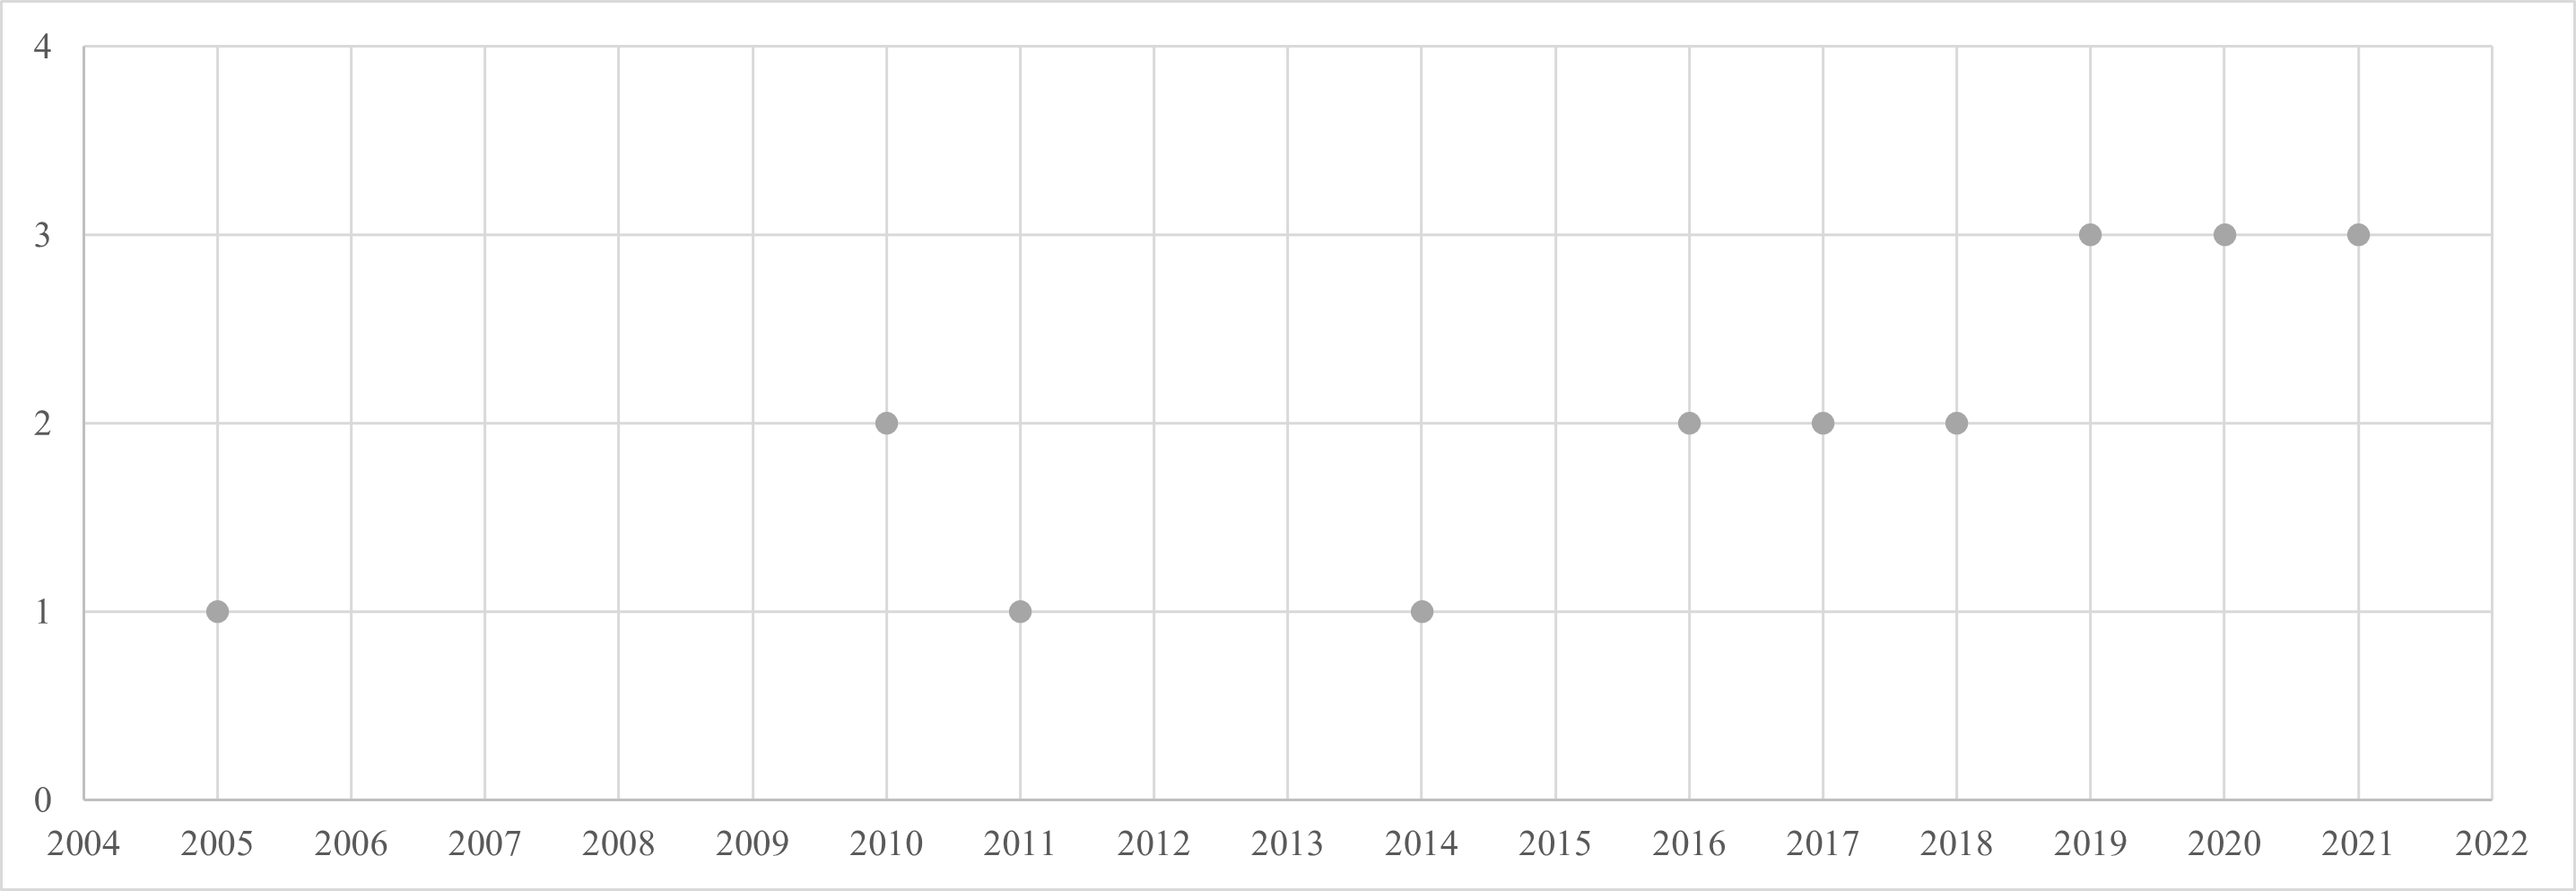
\includegraphics[width=\textwidth]{media/kappalemaarat-julkaisuvuosittain.png}
    \caption{Artikkeleiden kappalemäärät julkaisuvuosittain}
    \label{kuvio:kappalemaarat-julkaisuvuosittain}
\end{figure}


\section{Perehdytyskäytännöt}

Artikkeleissa mainittiin yhteensä 45 erilaista perehdytyskäytäntöä. Kuviossa \ref{kuvio:kaytannot} esitellään kukin käytäntö sekä niiden esiintymismäärät. Mentorointi mainittiin kuudessatoista artikkelissa tulokkaiden perehdytyskäytäntönä. Katselmointi (eng. code review) mainittiin yhdeksässä artikkelissa, kuten myös yhteistoiminnallinen ohjelmointi (pari- tai ryhmäohjelmointi). Organisaation sisäiseen dokumentaatioon perehtyminen oli kirjattu käytännöksi seitsemään eri artikkeliin. Tulokkaiden toiminta vertaisryhmänä, työtehtävän kontekstualisointi ja erilaiset tarkistuslistat saivat kukin viisi mainintaa, kuten myös "Good First Issue", joka viittaa työtehtävään, joka on ennakolta määritelty tulokkaille erityisen hyvin sopivaksi.

\begin{figure}[h]
    \centering
    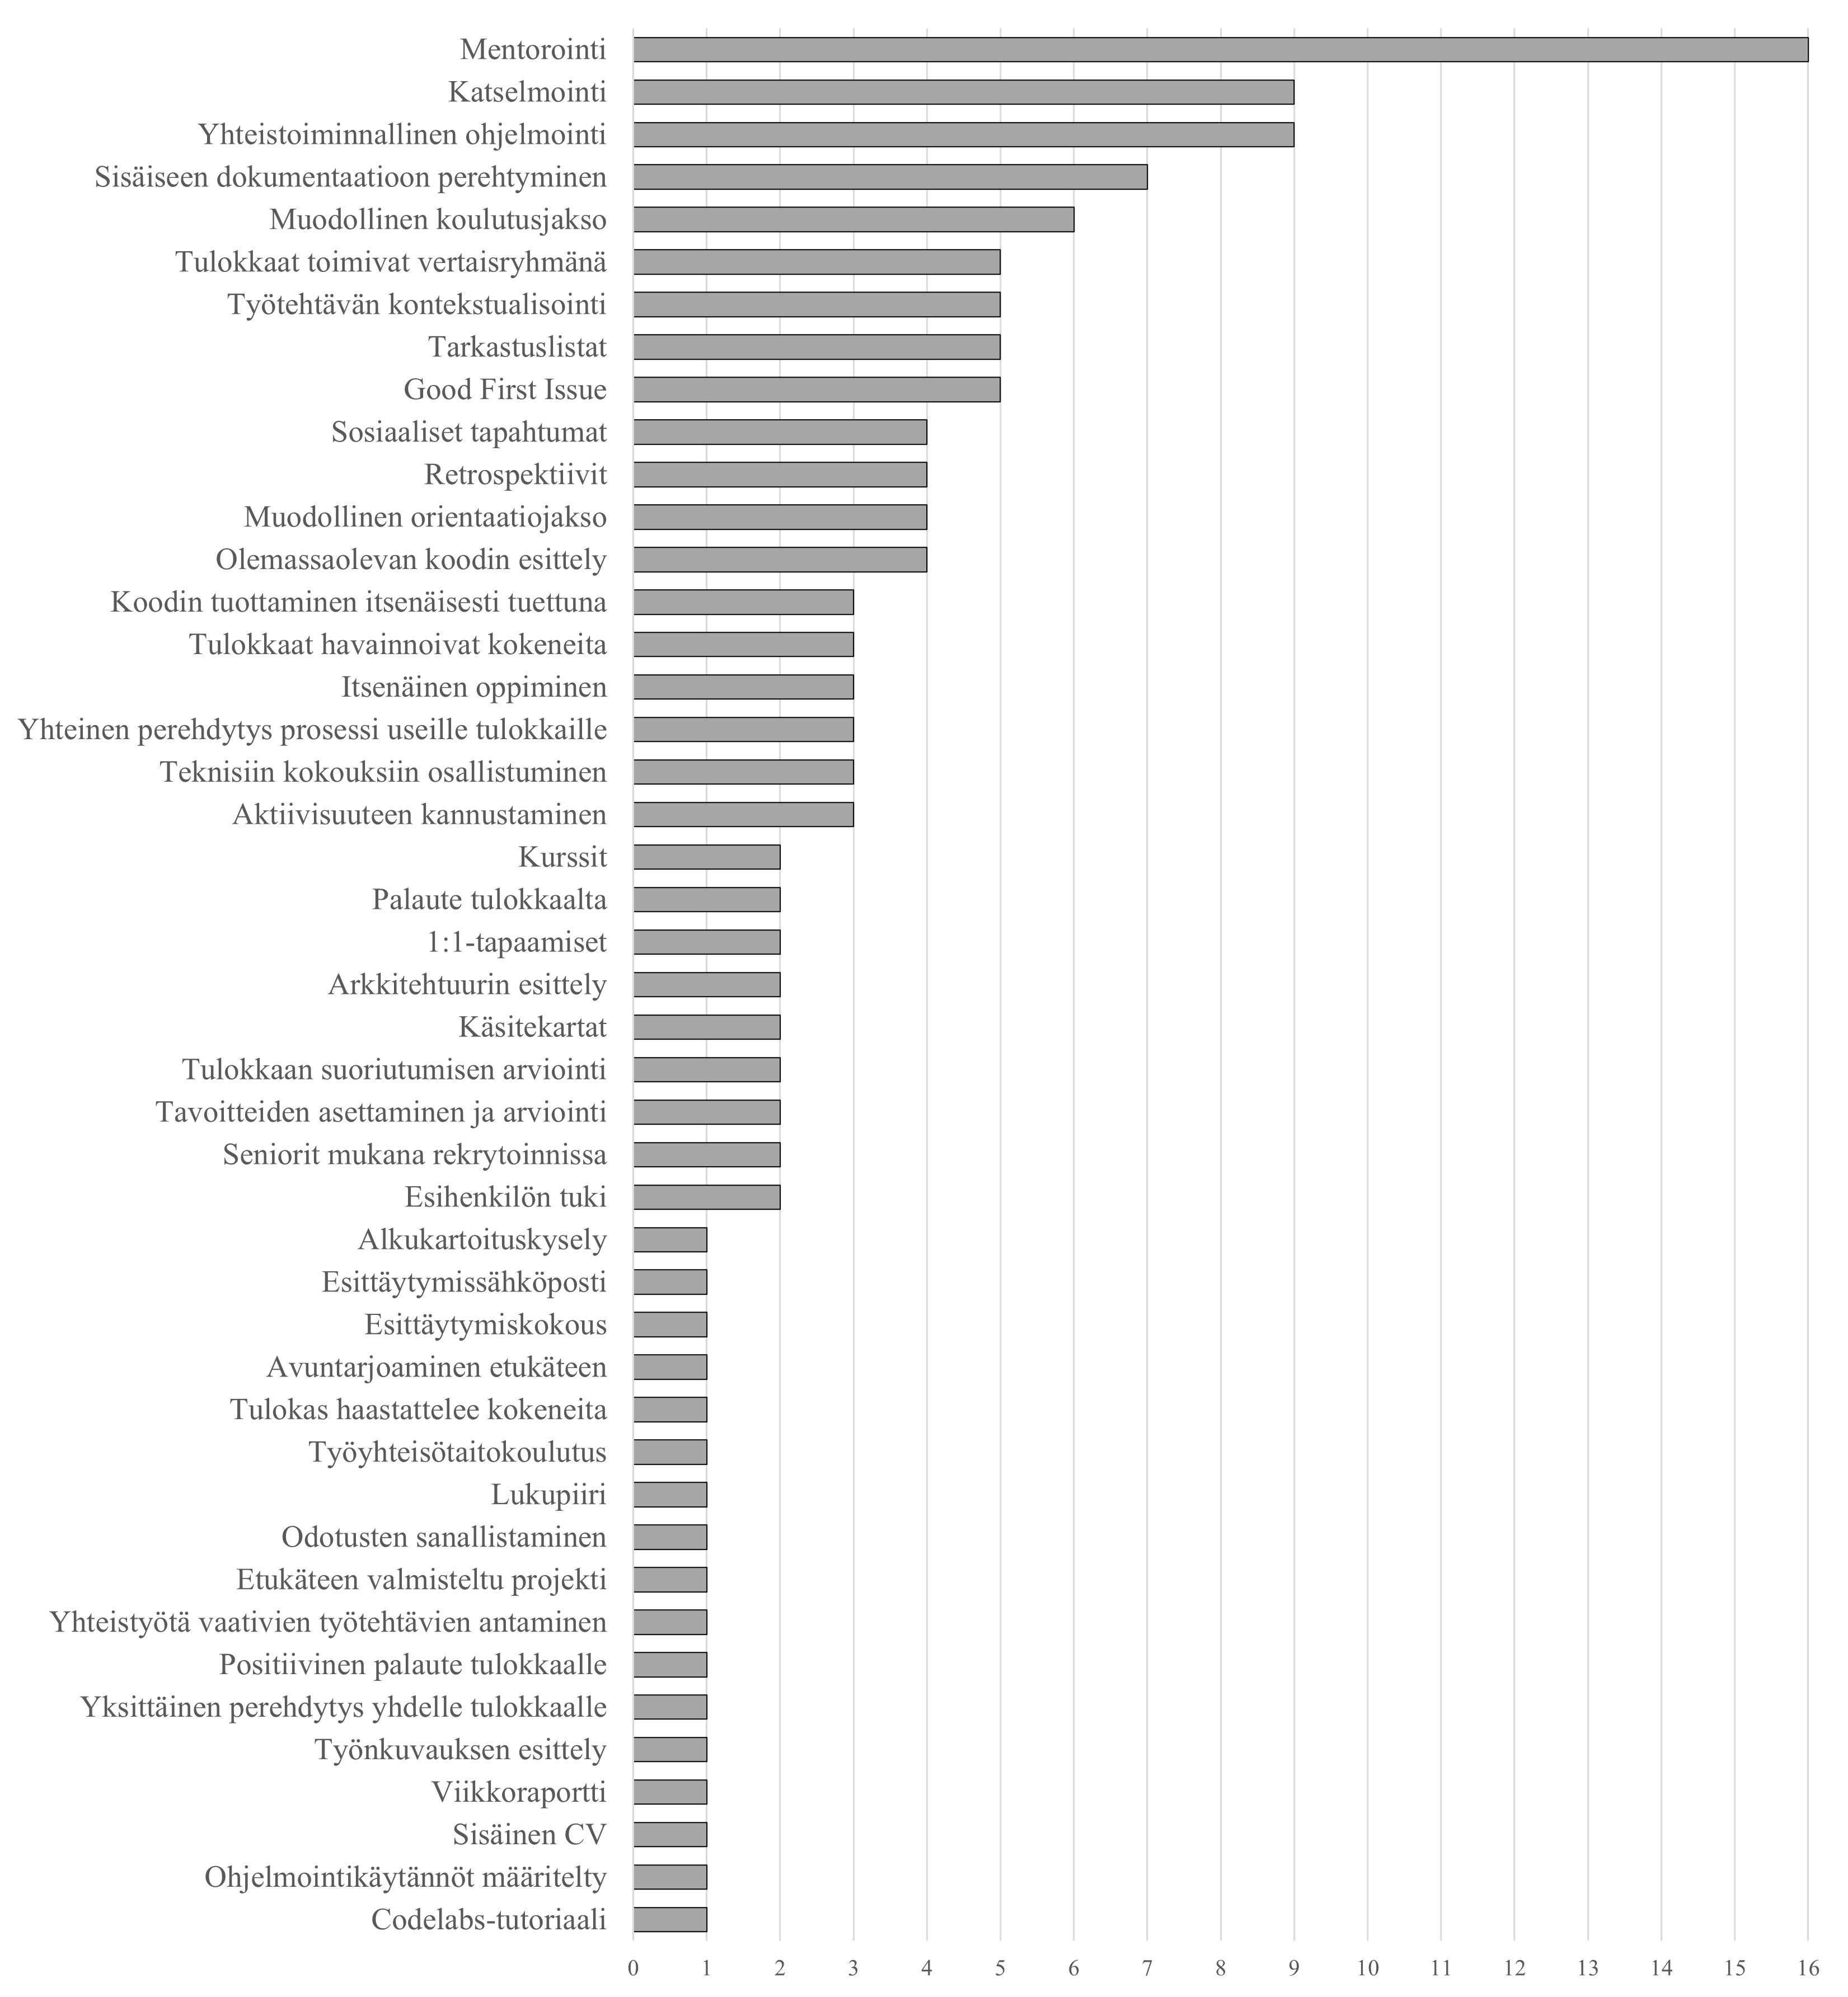
\includegraphics[width=\textwidth]{media/45-kaytannot.png}
    \caption{Perehdyttämiskäytännöt esiintymismäärineen}
    \label{kuvio:kaytannot}
\end{figure}

Löydettyjä perehdyttämiskäytäntöjä jaoteltiin luvussa \ref{luku-SRT-teoria} esitellyn sosialisaatioresurssien mukaisesti. Esimerkiksi sosialisaatioresurssien teorian ulottuvuuteen "1. Ennakoiva sosialisaatio" sijoitettiin alkukartoituskyselyihin ja esittäytymissähköposteihin liittyvät. Ulottuvuuksien mainintamäärät on kuvattu kuviossa \ref{kuvio:ulottuvuudet}. Mentoroinnin ulottuvuus oli yleisin, sillä se
mainittiin kuudessatoista artikkelissa. Ulottuvuus 12 (työtehtävät ja työn luonne) mainittiin viidessätoista. Tähän ulottuvuuden luettiin perehdyskäytäntöjä, jotka liittyivät läheisesti tulokkaan työtehtävien tekemiseen käytännössä - esimerkiksi tulokkaalle etukäteen valmistellut projektit, tulokkaan laatimat viikkoraportit ja teknisiin kokouksiin osallistuminen. Seuraavaksi eniten mainintoja sai palautteen ulottuvuus (11 artikkelia), johon luettiin katselmointi, tulokkaalle annettava positiivinen palaute ja tulokkaan suoriutumisen arviointi.

Neljä perehdytyskäytännöistä taas liittyivät selvästi orientaatiovaiheen jälkeiseen tulokkaisen keskinäiseen yhteistoiminnalliseen oppimiseen. Näissä käytännöissä samaan aikaan organisaatioon liittyneet tulokkaat toimivat siis yhdessä. Heille saatettiin antaa yhteistyötä vaativia työtehtäviä. Eräässä organisaatiossa yksi perehdytyskäytännöistä oli lukupiiri, jossa käsiteltiin ohjelmistokehitykseen liittyviä artikkeleita. Nämä yhteistoiminnallista oppimista edistävät käytännöt olen sijoittanut ulottuvuuteen 18, joka täydentää sosialisaatioresurssien teorian seitsemäätoista ulottuvuutta. Kuten kuviosta \ref{kuvio:ulottuvuudet} nähdään, tämä ulottuvuus on neljäntenä mainintojen määrällä mitattuna. Siihen kuuluvia käytäntöjä on mainittu yhdeksässä artikkelissa. 

Viisi perehdytyskäytäntöä eivät olleet luokiteltavissa yhteen sosialisaatioresurssien teorian ulottuvuuteen. Nämä olivat mm. sisäinen CV (jolla tulokkaat tekivät omaa osaamistaan näkyväksi, mutta myös saivat tietoa kollegoidensa osaamisesta), tulokkaiden tekemä kokeneiden työntekijöiden havainnointi sekä kokeneiden työntekijöiden mukanaolo rekrytointiprosessissa. 

\begin{figure}[h]
    \centering
    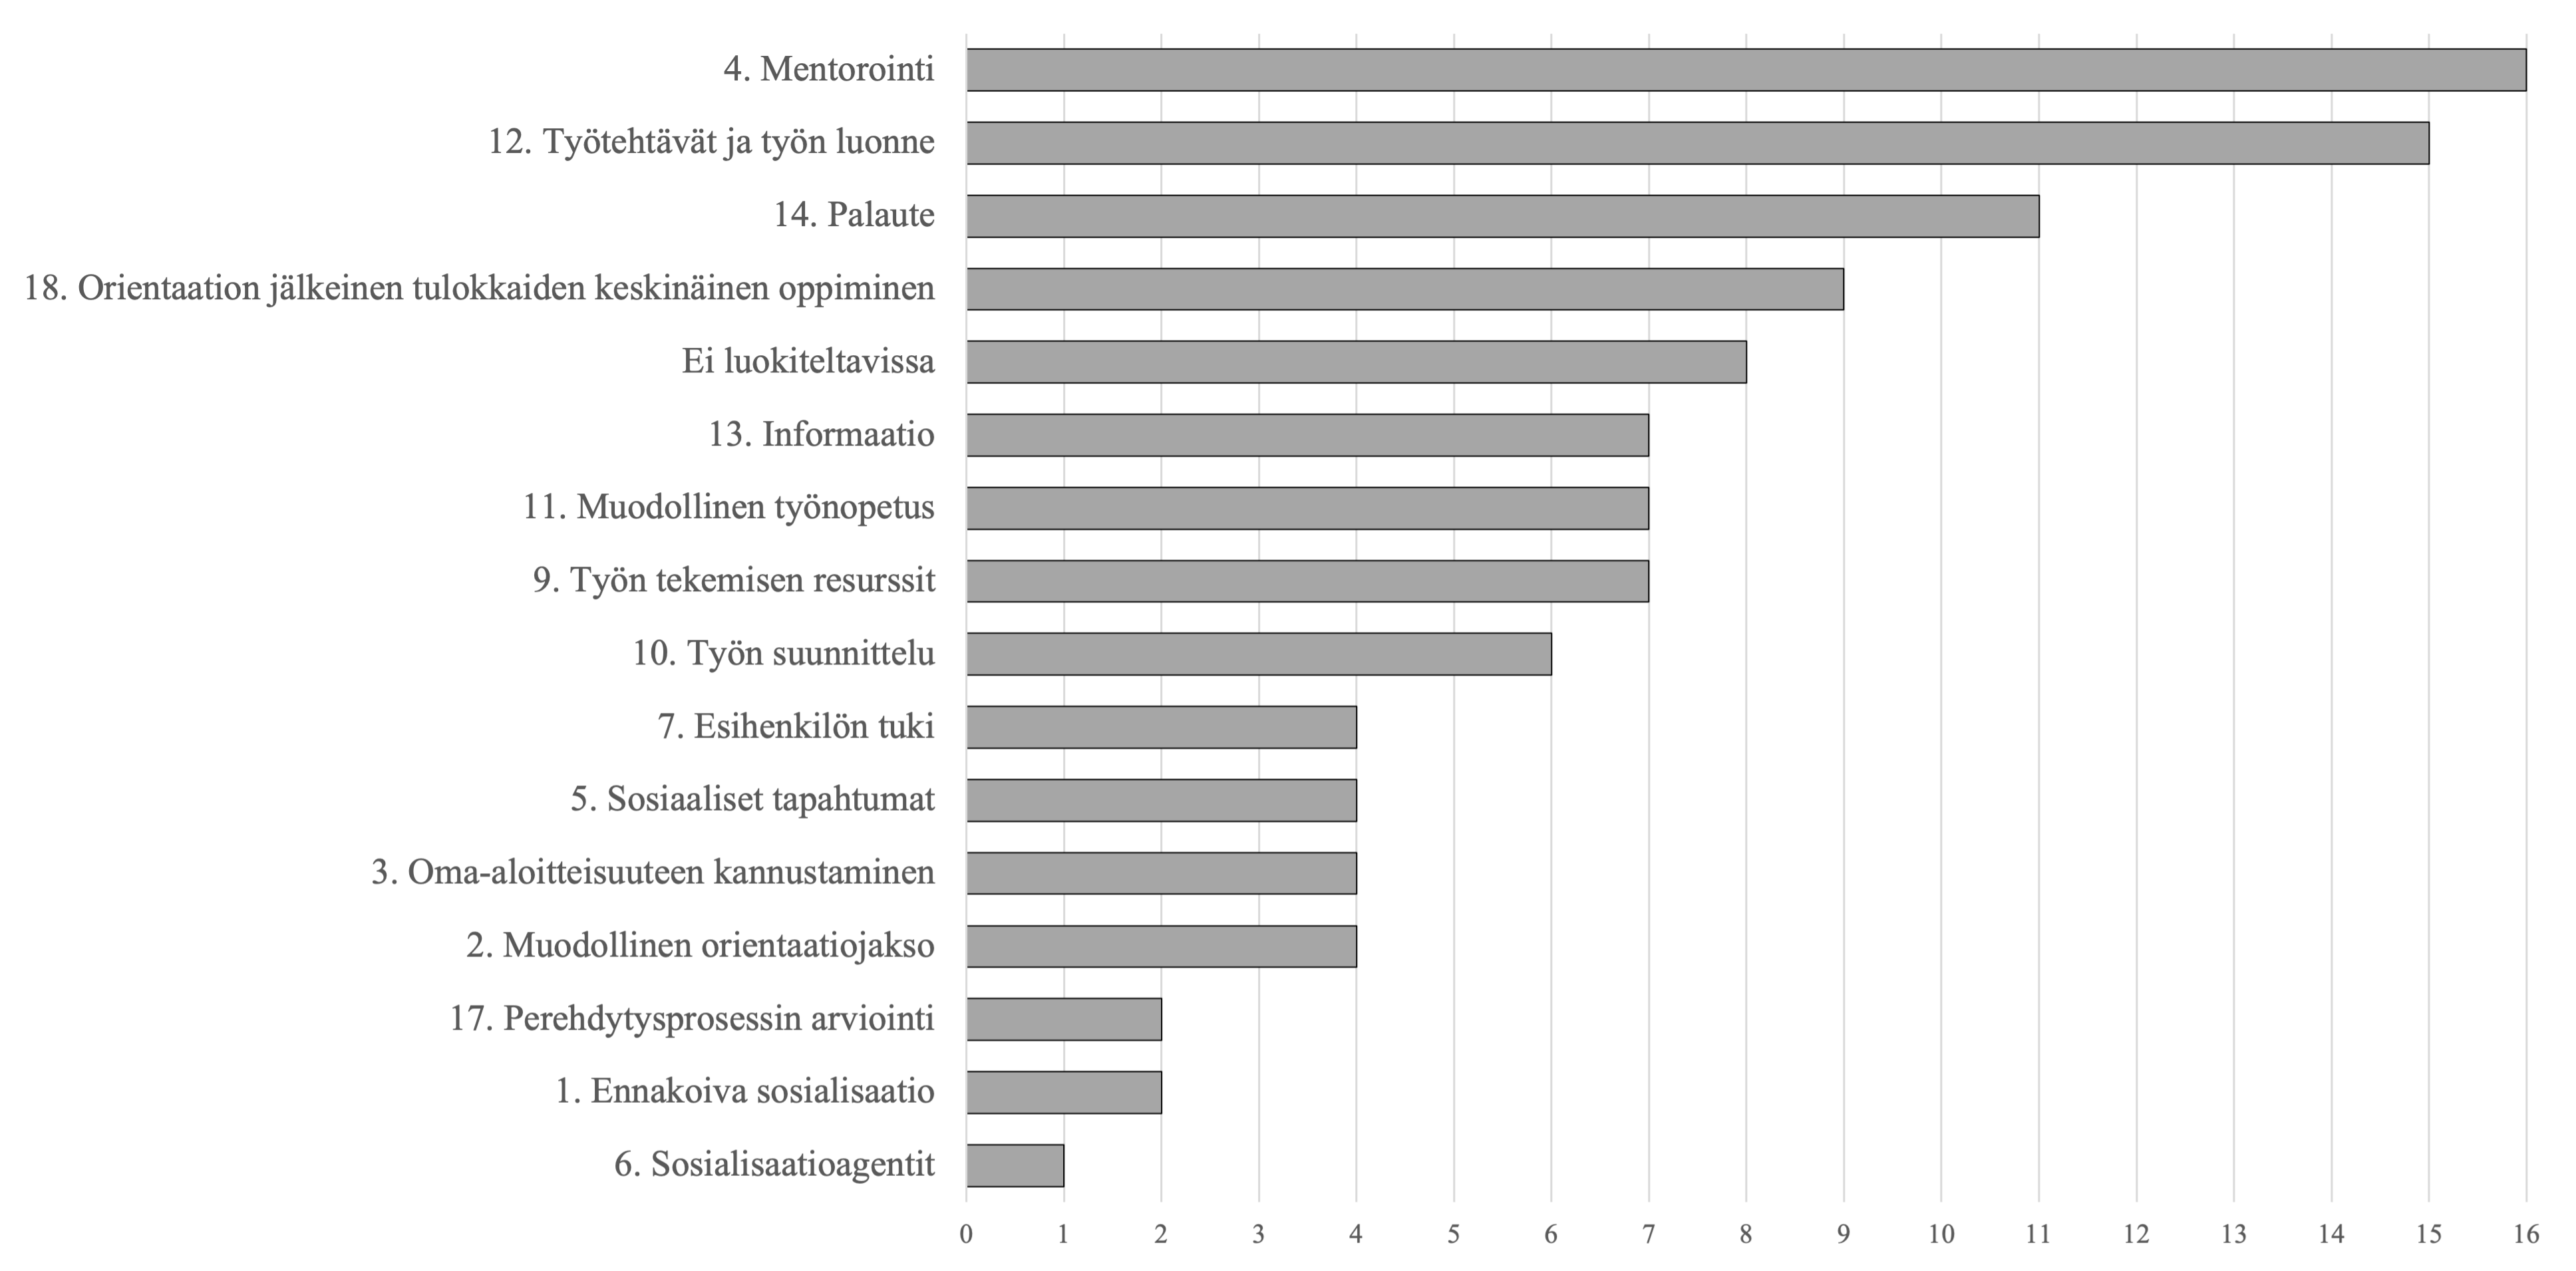
\includegraphics[width=\textwidth]{media/ulottuvuudet.png}
    \caption{Perehdyttämiskäytännöt esiintymismäärineen jaoteltuna sosialisaatioresurssien \parencite{saks-gruman-2012} mukaan}
    \label{kuvio:ulottuvuudet}
\end{figure}

todo nimeä matriisi + viittaa + kirjoita tekstiä

\begin{adjustbox}{width=\textwidth,totalheight=\textheight,keepaspectratio}
\begin{tabularx}{\linewidth}{@{}>{\RaggedRight}p{1.5cm}X@{}}
\toprule
\textbf{Nro} & \textbf{Sosialisaatioresurssiulottuvuus} \\
\midrule
1 & Ennakoiva sosialisaatio \\
2 & Muodollinen orientaatiojakso \\
3 & Oma-aloitteisuuteen kannustaminen \\
4 & Mentorointi \\
5 & Sosiaaliset tapahtumat \\
6 & Sosialisaatioagentit \\
7 & Esihenkilön tuki \\
9 & Työn tekemisen resurssit \\
10 & Työn suunnittelu \\
11 & Muodollinen työnopetus \\
12 & Työtehtävät ja työn luonne \\
13 & Informaatio \\
14 & Palaute \\
17 & Perehdytysprosessin arviointi \\
18 & Orientaation jälkeinen tulokkaiden keskinäinen oppiminen \\
\bottomrule
\caption{Kuvion \ref{tbl:ulottuvuusmatriisi} selite: sosialisaatioresurssiulottuvuudet}
\label{tbl:ulottuvuusmatriisin-selite}
\end{tabularx}

\end{adjustbox}


\begin{adjustbox}{width=\textwidth,totalheight=\textheight,keepaspectratio}
\small
\begin{tabularx}{\linewidth}{@{}>{\RaggedRight}p{5.5cm}*{16}{X}@{}}
\toprule
\textbf{Artikkeli} & \textbf{1} & \textbf{2} & \textbf{3} & \textbf{4} & \textbf{5} & \textbf{6} & \textbf{7} & \textbf{9} & \textbf{10} & \textbf{11} & \textbf{12} & \textbf{13} & \textbf{14} & \textbf{17} & \textbf{18} \\

\midrule
\textcite{rodeghero-ym-2021} & 0 & 0 & 0 & 0 & 0 & 0 & 0 & 0 & 0 & 0 & 0 & 0 & 0 & 0 & 0 \\
\midrule
\textcite{azanza-ym-2021} & 0 & 0 & 0 & 0 & 0 & 0 & 0 & 0 & 0 & 0 & 0 & 0 & 0 & 0 & 0 \\
\midrule
\textcite{ju-ym-2021} & 0 & 0 & 0 & 0 & 0 & 0 & 0 & 0 & 0 & 0 & 0 & 0 & 0 & 0 & 0 \\
\midrule
\textcite{britto-ym-2020} & 0 & 0 & 0 & 0 & 0 & 0 & 0 & 0 & 0 & 0 & 0 & 0 & 0 & 0 & 0 \\
\midrule
\textcite{yates-ym-2020} & 0 & 0 & 0 & 0 & 0 & 0 & 0 & 0 & 0 & 0 & 0 & 0 & 0 & 0 & 0 \\
\midrule
\textcite{moe-ym-2020} & 0 & 0 & 0 & 0 & 0 & 0 & 0 & 0 & 0 & 0 & 0 & 0 & 0 & 0 & 0 \\
\midrule
\textcite{kumar-wallace-2019} & 0 & 0 & 0 & 0 & 0 & 0 & 0 & 0 & 0 & 0 & 0 & 0 & 0 & 0 & 0 \\
\midrule
\textcite{viviani-murphy-2019} & 0 & 0 & 0 & 0 & 0 & 0 & 0 & 0 & 0 & 0 & 0 & 0 & 0 & 0 & 0 \\
\midrule
\textcite{buchan-ym-2019} & 0 & 0 & 0 & 0 & 0 & 0 & 0 & 0 & 0 & 0 & 0 & 0 & 0 & 0 & 0 \\
\midrule
\textcite{tuzun-ym-2018} & 0 & 0 & 0 & 0 & 0 & 0 & 0 & 0 & 0 & 0 & 0 & 0 & 0 & 0 & 0 \\
\midrule
\textcite{matturro-ym-2017} & 0 & 0 & 0 & 0 & 0 & 0 & 0 & 0 & 0 & 0 & 0 & 0 & 0 & 0 & 0 \\
\midrule
\textcite{britto-ym-2017} & 0 & 0 & 0 & 0 & 0 & 0 & 0 & 0 & 0 & 0 & 0 & 0 & 0 & 0 & 0 \\
\midrule
\textcite{pham-ym-2017} & 0 & 0 & 0 & 0 & 0 & 0 & 0 & 0 & 0 & 0 & 0 & 0 & 0 & 0 & 0 \\
\midrule
\textcite{kumar-ym-2016} & 0 & 0 & 0 & 0 & 0 & 0 & 0 & 0 & 0 & 0 & 0 & 0 & 0 & 0 & 0 \\
\midrule
\textcite{shannon-pool-2016} & 0 & 0 & 0 & 0 & 0 & 0 & 0 & 0 & 0 & 0 & 0 & 0 & 0 & 0 & 0 \\
\midrule
\textcite{viana-ym-2014} & 0 & 0 & 0 & 0 & 0 & 0 & 0 & 0 & 0 & 0 & 0 & 0 & 0 & 0 & 0 \\
\midrule
\textcite{hemphill-begel-2011} & 0 & 0 & 0 & 0 & 0 & 0 & 0 & 0 & 0 & 0 & 0 & 0 & 0 & 0 & 0 \\
\midrule
\textcite{kulkarni-ym-2010} & 0 & 0 & 0 & 0 & 0 & 0 & 0 & 0 & 0 & 0 & 0 & 0 & 0 & 0 & 0 \\
\midrule
\textcite{johnson-senges-2010} & 0 & 0 & 0 & 0 & 0 & 0 & 0 & 0 & 0 & 0 & 0 & 0 & 0 & 0 & 0 \\
\midrule
\textcite{bjornson-dingsøyr-2005} & 0 & 0 & 0 & 0 & 0 & 0 & 0 & 0 & 0 & 0 & 0 & 0 & 0 & 0 & 0 \\
\bottomrule
\caption{Artikkeleissa ilmenneet sosialisaatioresurssiulottuvuudet}
\label{tbl:ulottuvuusmatriisi}
\end{tabularx}

\end{adjustbox}

TODO Montako käytäntöä keskimäärin löydettiin havainnoimalla?

TODO Montako käytäntöä keskimäärin löydettiin kyselyillä?


\section{Tutkimustyypit ja -menetelmät}
\label{luku-tutkimustyypit-ja-menetelmat}

Katsaukseen valituissa artikkeleissa raportoitiin erilaista tutkimuksista (ks. \ref{kuvio:tutkimustyypit}). Kolmessatoista artikkelissa oli hyödynnetty yhtä tutkimustyyppiä ja seitsemässä kahta tai kolmea. Esimerkiksi \textcite{azanza-ym-2021} tutkivat kyselytutkimuksen avulla käsitekarttojen käyttämistä tulokkaiden perehdyttämisessä, kun taas \textcite{pham-ym-2017} toteuttivat eksploratiivisen haastattelu- ja kyselytutkimuksen. Aineiston artikkeleissa eniten oli toteutettu tapaustutkimuksia (yhdeksän). Kyselyt ja haastattelut mainittiin viidessä artikkelissa. Kolme tutkimusta luokiteltiin eksploratiiviseksi. Toimintatutkimuksia oli kaksi: \textcite{bjornson-dingsøyr-2005} kehittivät tutkimuksessaan konsulttiyrityksen mentorointikäytäntöjä toteuttamalla alkuhaastatteluja ja kirjallisuuskatsauksen, joiden perusteella mentorointiohjelma uudistettiin. Immersiivisestä etnografiasta raportoivia artikkeleita aineistossa oli kaksi. \textcite{kumar-ym-2016} raportoivat tutkimuksesta, jossa tutkija työskenteli kohdeyrityksessä ohjelmistokehittäjänä kahdeksan kuukauden ajan käyttäen havainnointia ja haastattelua tutkimusmenetelminä. Saman tutkimusryhmän artikkeli \textcite{kumar-wallace-2019} perustuu samaan aineistoon. 

\begin{figure}[h]
    \centering
    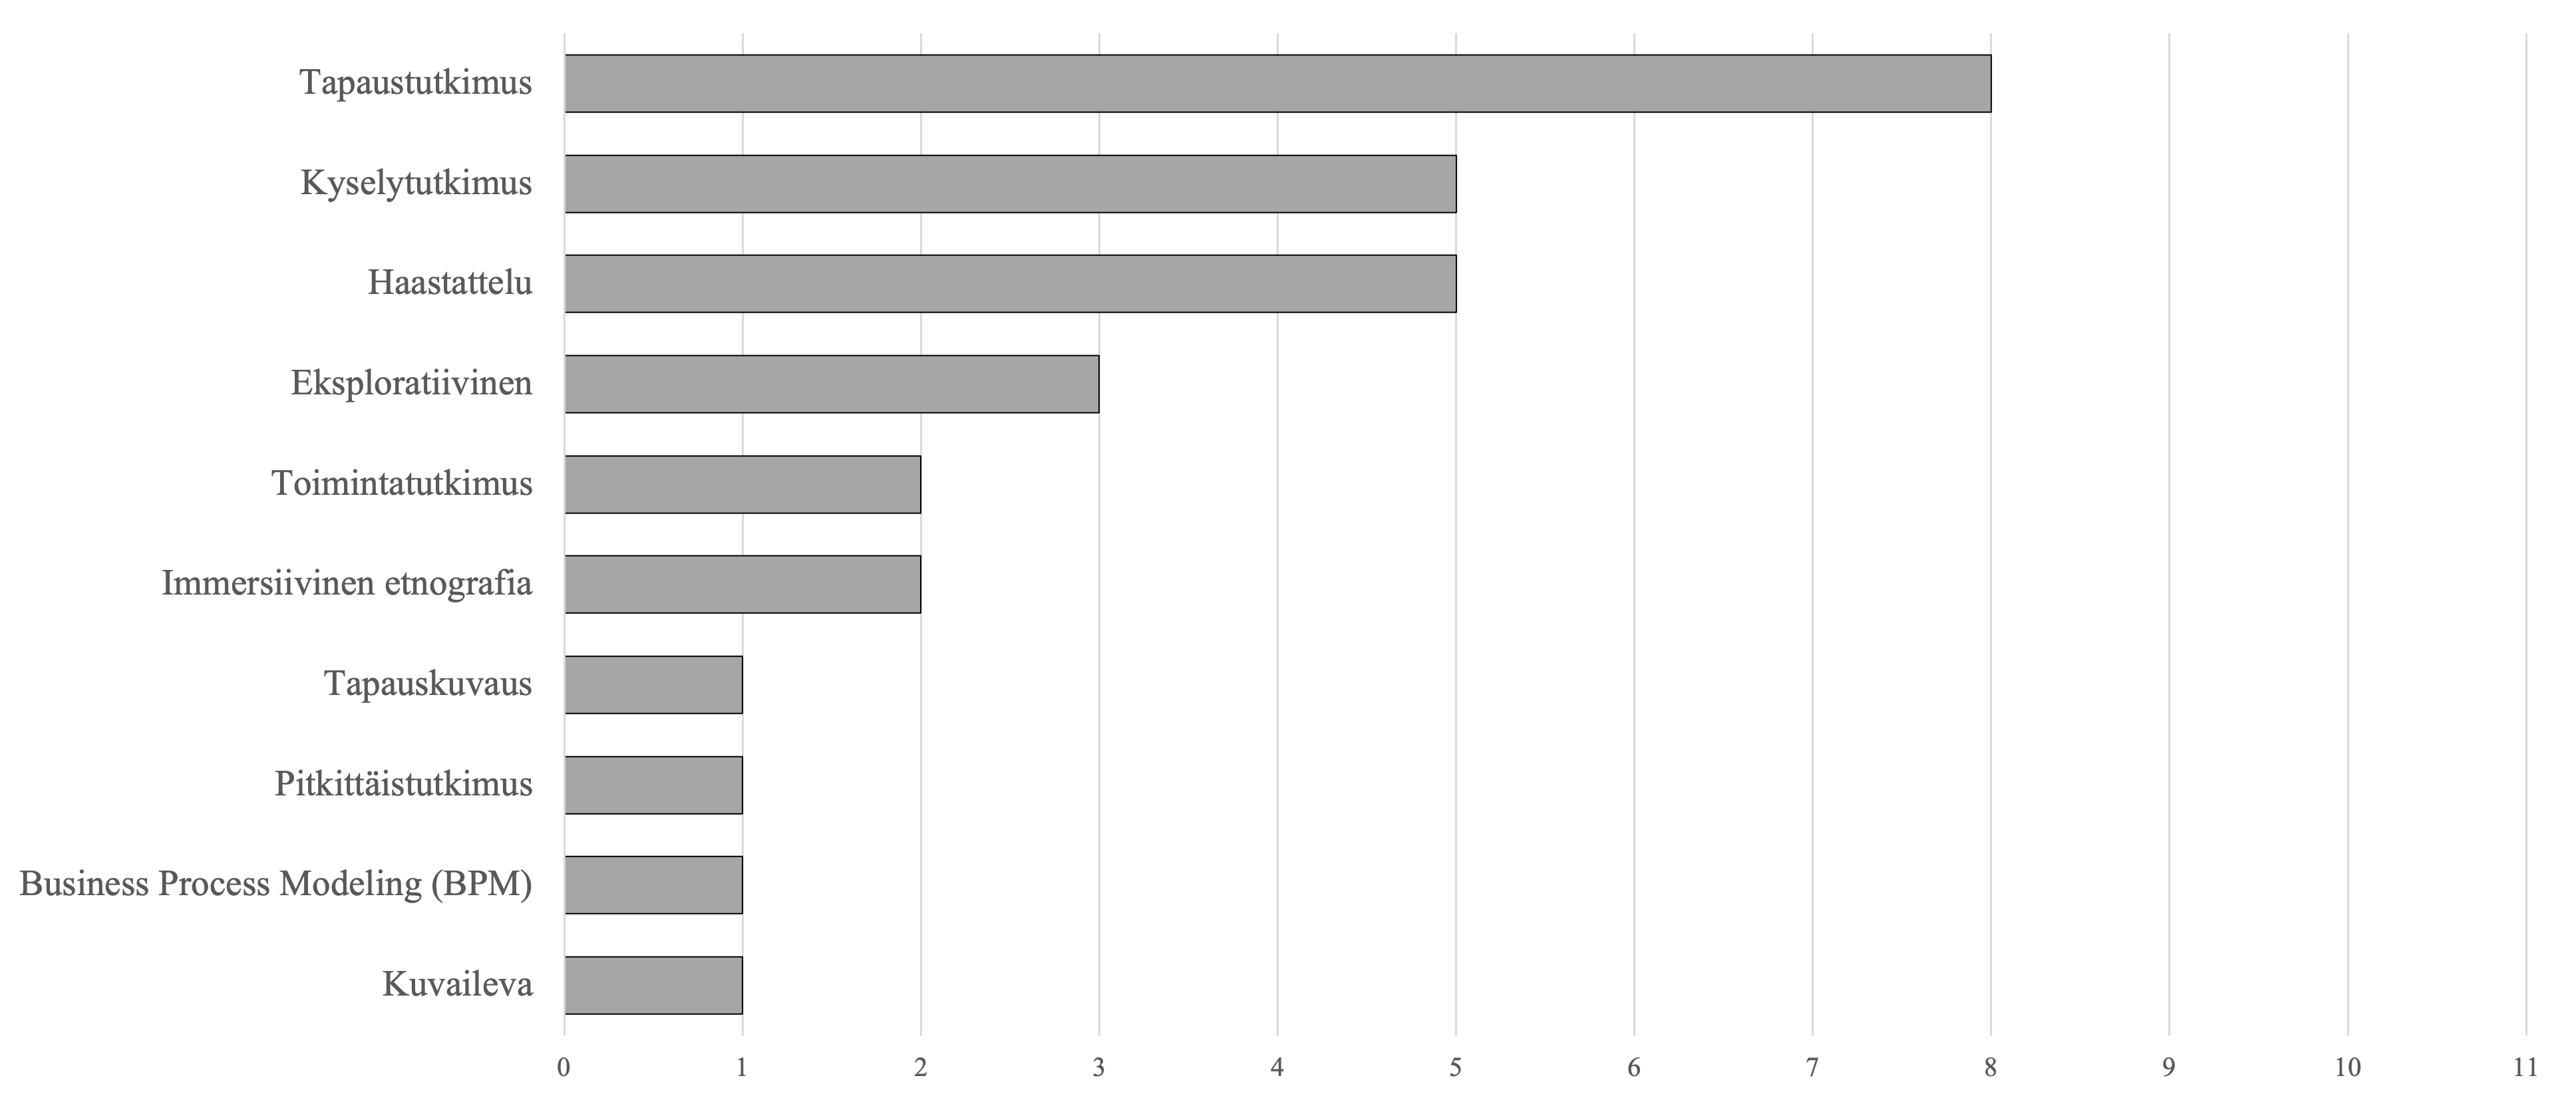
\includegraphics[width=\textwidth]{media/tutkimustyypit.png}
    \caption{Artikkeleissa ilmenneet tutkimustyypit}
    \label{kuvio:tutkimustyypit}
\end{figure}

Artikkeleissa mainittiin yhteensä 12 eri tutkimusmenetelmää (\ref{kuvio:tutkimusmenetelmat}). Eniten käytetty oli puolistrukturoitu haastattelu, jota käytettiin yhdentoista artikkelin tutkimuksessa. Kyselyä taas käytettiin seitsemässä: esimerkiksi \textcite{kulkarni-ym-2010} toteuttivat kyselyt vastavalmistuneille ohjelmistokehittäjille ja ohjelmistoalan yritysten HR-asiantuntijoille saadakseen tietoa siitä, minkälaisia perehdytysohjelmia yrityksissä on. Aineistossa havainnointi (5) ja osallistuva havainnointi (2) saivat myös mainintoja. Grounded theory-menetelmä mainittiin neljässä artikkelissa. Esimerkiksi \textcite{viana-ym-2014} tutkivat sitä, miten ohjelmistokehitykseen liittyvä tieto siirtyy kokeneilta osaajilta vasta-alkajille. 

TODO luetellaanko myös loput, vähemmän käytetyt menetelmät?

\begin{figure}[h]
    \centering
    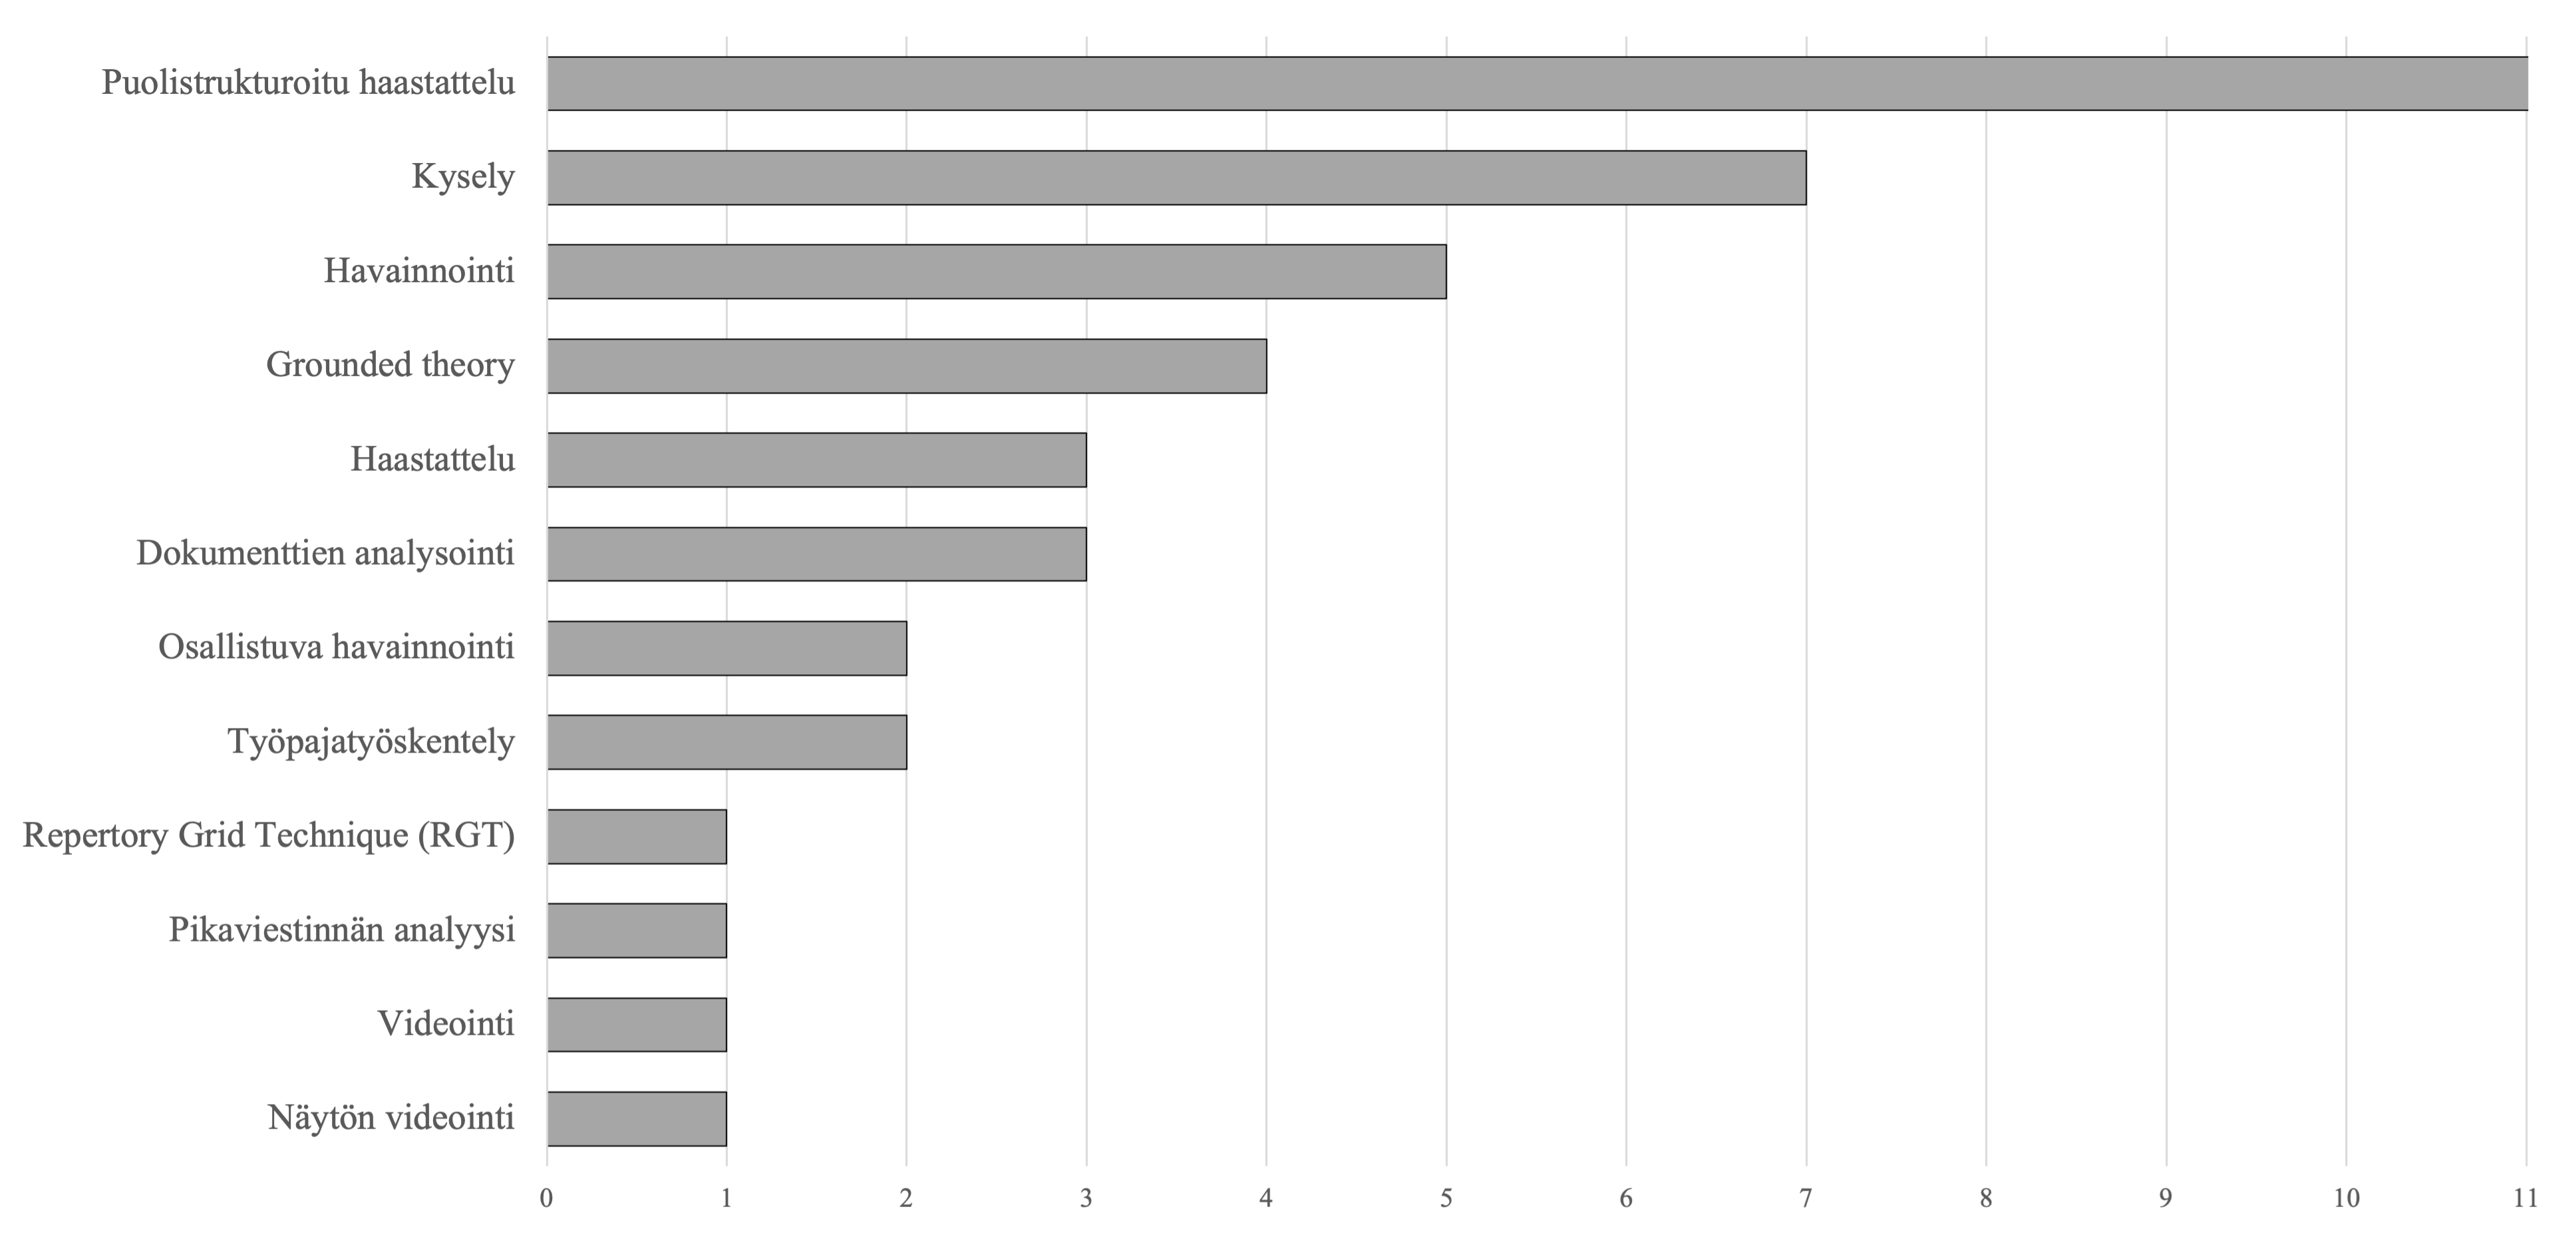
\includegraphics[width=\textwidth]{media/menetelmat.png}
    \caption{Artikkeleissa ilmenneet tutkimusmenetelmät}
    \label{kuvio:tutkimusmenetelmat}
\end{figure}

Tämän katsauksen tavoitteena oli siis selvittää, minkälaisia perehdytyskäytäntöjä ohjelmistoalan yrityksissä käytetään. Aineistosta voidaan havaita myös se, minkälaisten tutkimusmenetelmien käyttäminen johti erilaisiin perehdytyskäytäntömäärien löytämiseen

Aineiston perusteella voidaan tehdä havaintoja siitä, miten tutkimusmenetelmien valinta vaikutti löydettyjen perehdytyskäytäntöjen määrään. Kuviossa \ref{kuvio:menetelmilla-havaitut-kaytannot} on esitetty keskiarvot sille, montako perehdytyskäytäntöä keskimäärin mainittiin eri tutkimusmenetelmiä käyttäneissä artikkeleissa. Kuviosta voidaan havaita, että Repertory Grid Technique -menetelmän avulla käytäntöjä löytyi eniten (15). Myös pikaviestinnän (kahdeksan) ja dokumenttien (7) analysointi toi esiin useita käytäntöjä. Myös havainnointi tai osallistuva havainnointi (yht. 9,4) ja haastattelut (yht. 8,9) antoivat tietoa käytäntöjen määrästä. Videointi tai näytön videointi taas eivät olleet tehokkaita tapoja löytää käytäntöjä, sillä molemmilla löytyi keskimäärin yksi perehdytyskäytäntö.


\begin{figure}[h]
    \centering
    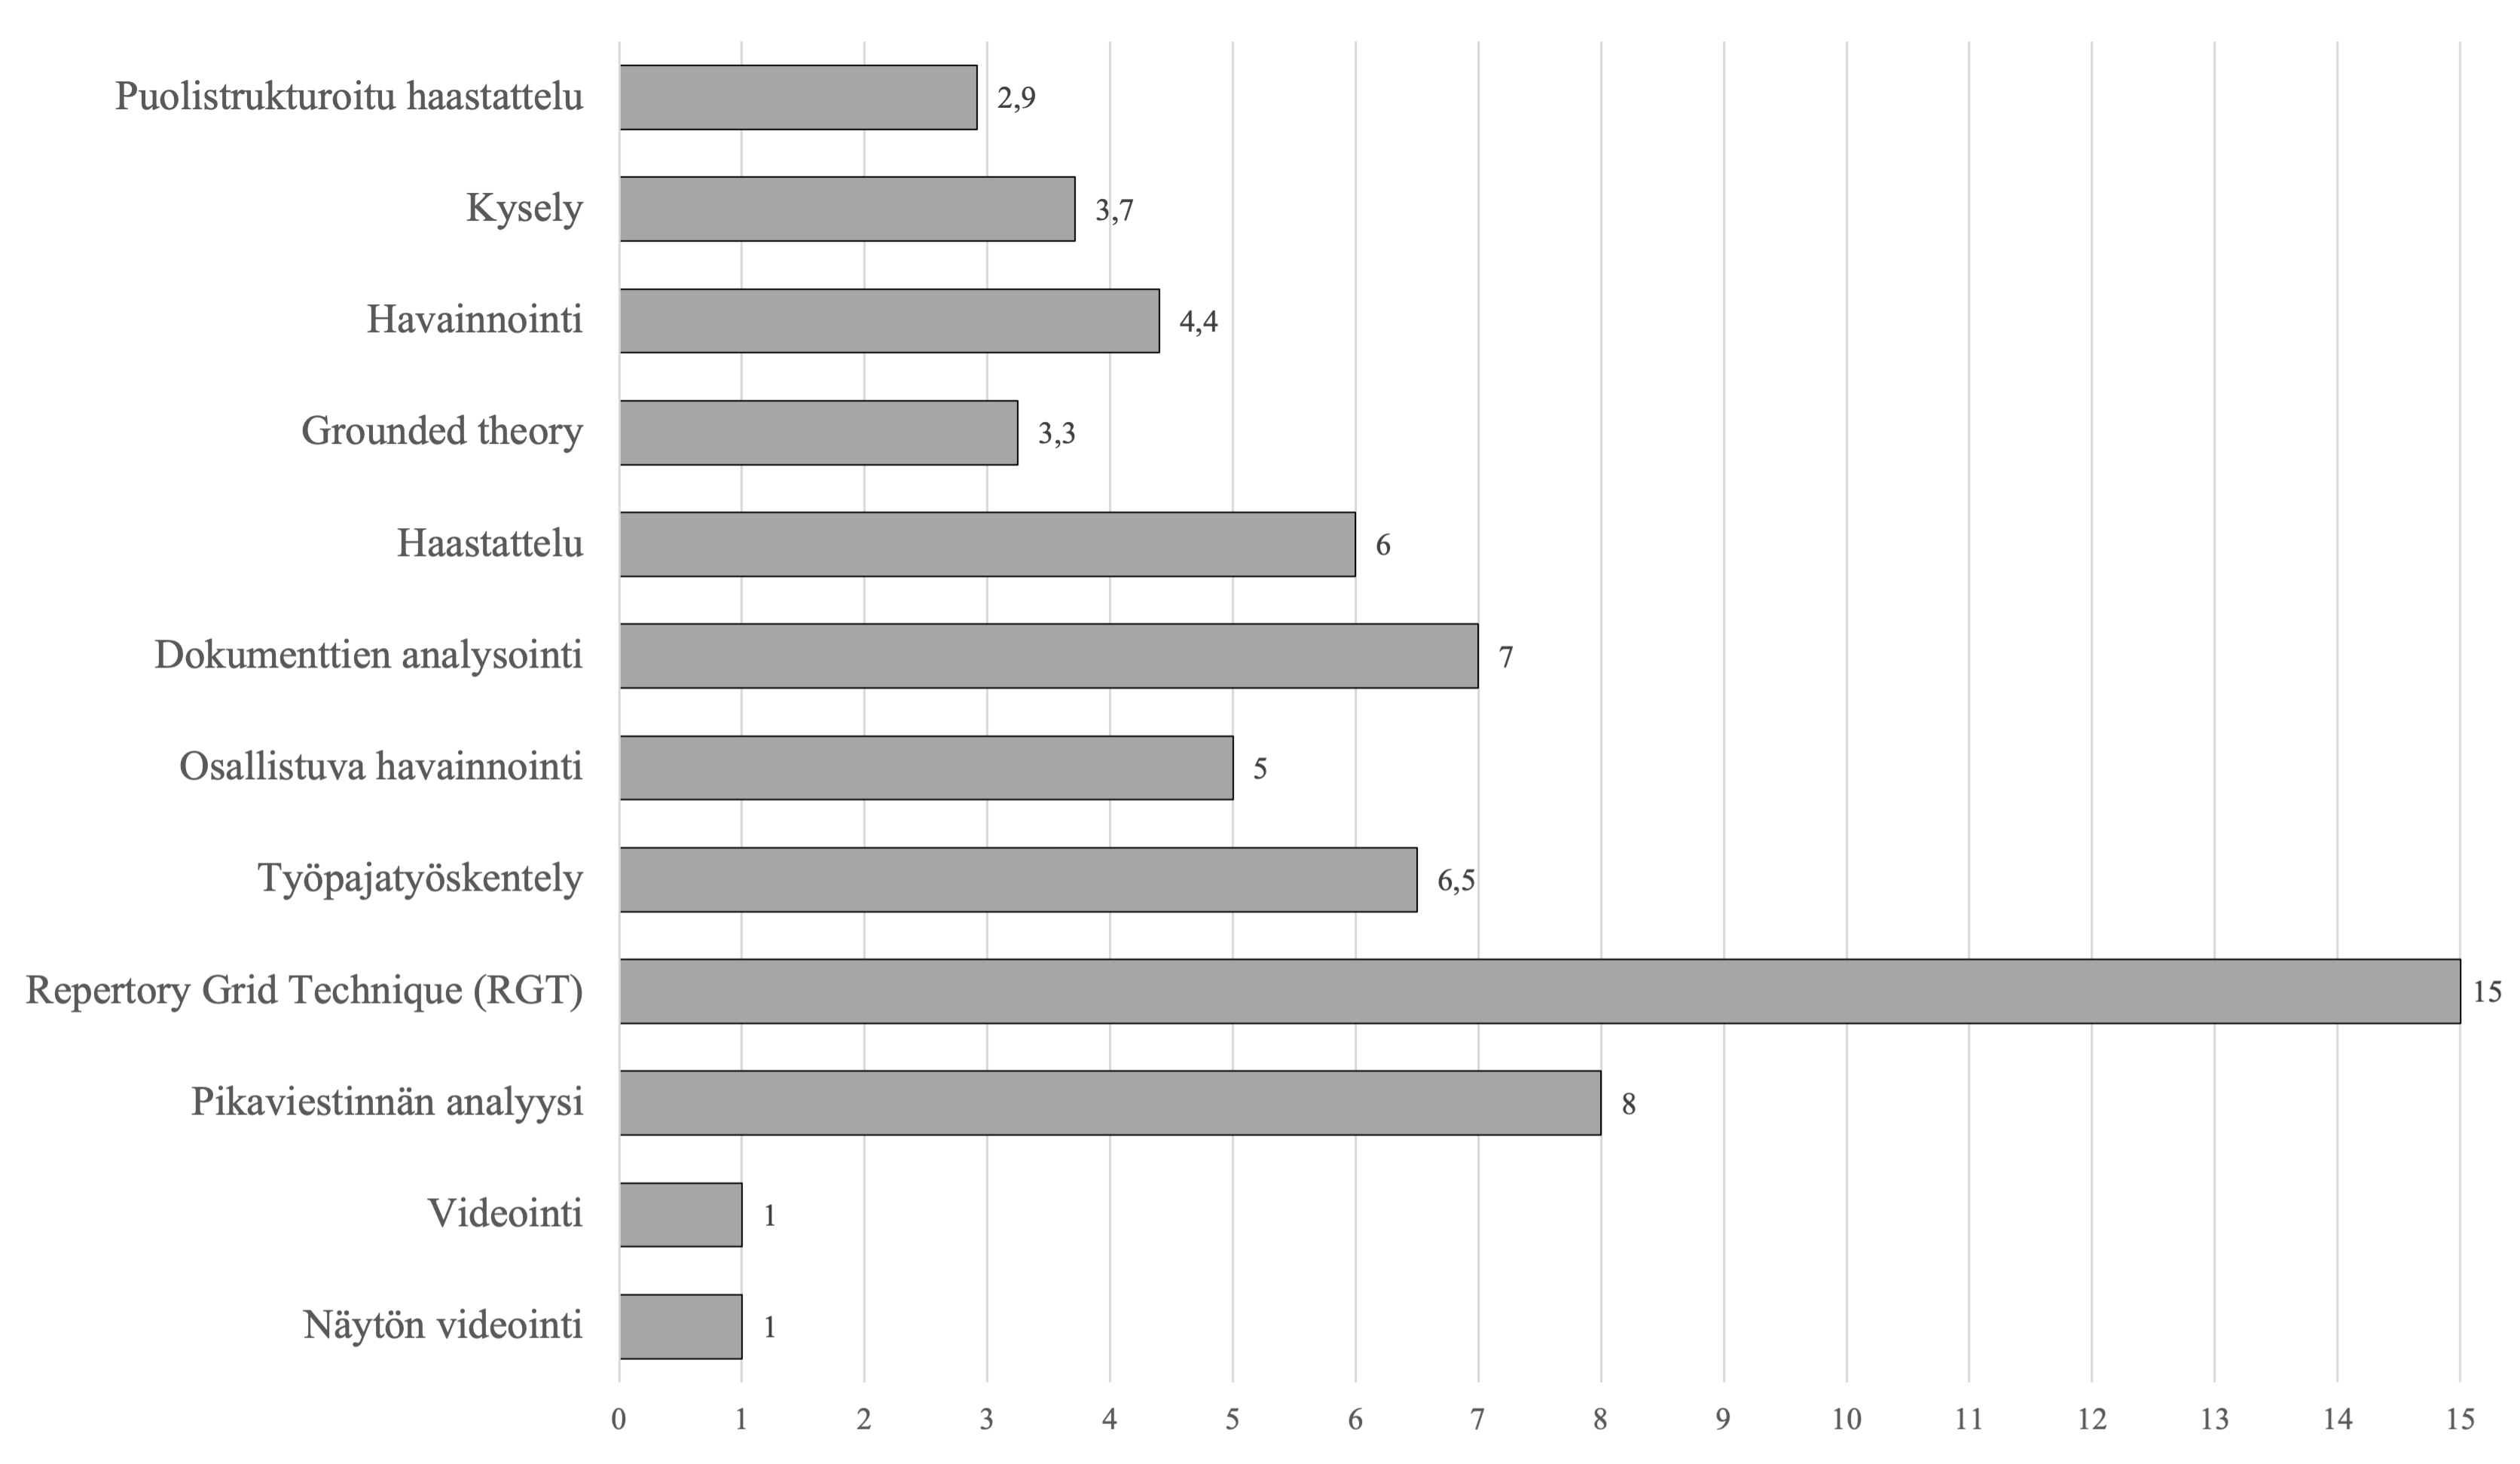
\includegraphics[width=\textwidth]{media/menetelmilla-havaitut-kaytannot.png}
    \caption{Keskiarvoiset artikkeleissa mainittujen perehdytyskäytäntöjen määrät tutkimusmenetelmittäin}
    \label{kuvio:menetelmilla-havaitut-kaytannot}
\end{figure}



\section{Tutkittavien organisaatioiden kontekstit}

Katsauksen artikkeleissa tutkitut yritykset toimivat eri konteksteissa (\ref{kuvio:kontekstit}). Eniten mainittu konteksti artikkeleissa oli Agile eli ketterät menetelmät, joka mainittiin seitsemässä artikkelissa kahdestakymmenestä. Seuraavaksi eniten, viisi mainintaa, saivat globaalisti hajautettu ohjelmistokehitys ja suuret yritykset. Esimerkiksi \textcite{johnson-senges-2010} kertovat Googlen sekä \textcite{rodeghero-ym-2021} \textcite{ju-ym-2021} Microsoftin perehdytyskäytännöistä. Etätyöskentely, pienet yritykset, yrityksen järjestämä akatemia ja keskikokoiset yritykset olivat kontekstina kukin kahdessa artikkelissa. Esimerkiksi \textcite{rodeghero-ym-2021} raportoivat koronapandemian aikana työnsä aloittaneiden ohjelmistokehittäjien perehdyttämisestä.

\begin{figure}[h]
    \centering
    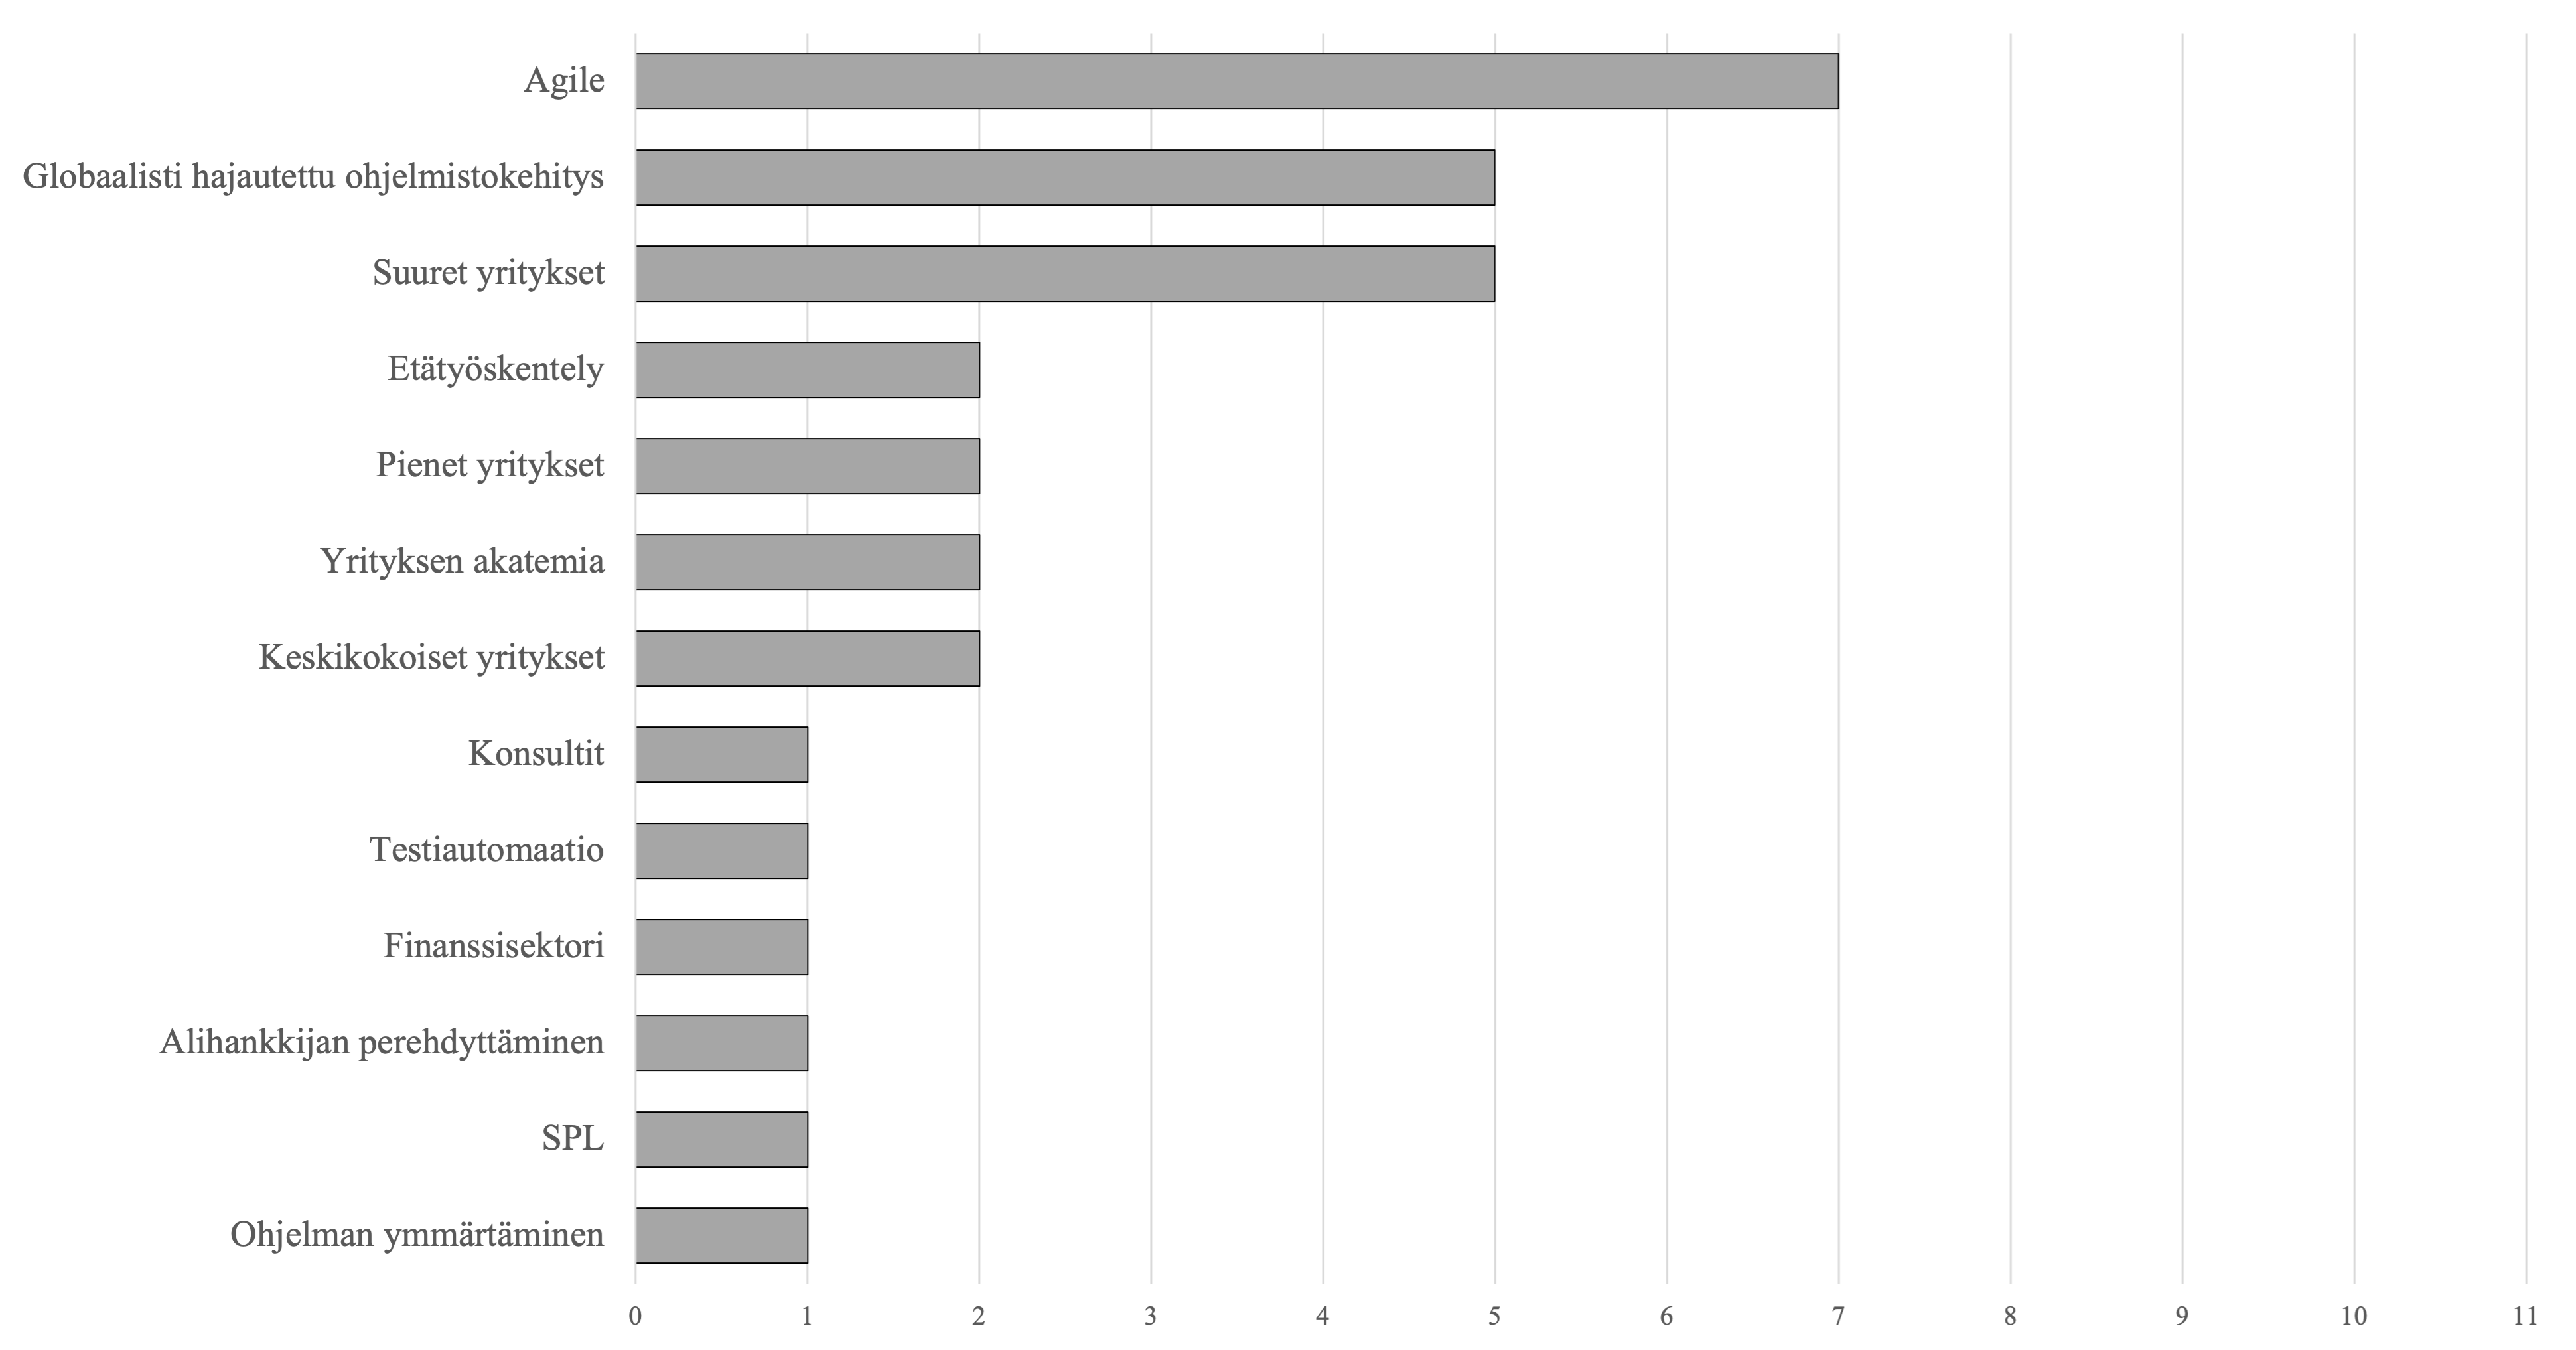
\includegraphics[width=\textwidth]{media/kontekstit.png}
    \caption{Artikkeleissa ilmenneet kontekstit}
    \label{kuvio:kontekstit}
\end{figure}


...
\chapter{Päätäntä}
...
\section{Yhteenveto / johtopäätökset}
...
\section{Jatkotutkimusaiheet}

Tässä tutkimuksessa perehdyttämistä tarkasteltiin nimenomaan organisaation tai sen edustajien aloitteesta tapahtuvan toiminnan näkökulmasta. Kuitenkin myös uuden työntekijän omalla toiminnalla on vaikutusta työhön perehtymiseen, mitä olisi hyvä myös tutkia.

% Tavoitteiden asettaminen ja arviointi mainittiin vain 10%:ssä! Vaikka minkäs tulosten mukaan se olisi tosi tärkeää? Tästä hyvä jatkotutkimusaihe
...

\section{Eettiset ulottuvuudet}

...

\section{Arviointi}
...

Artikkeleita arvioi siis ainoastaan yksi henkilö, tutkimuksen laatija. Näin ollen henkilökohtainen näkemys on saattanut vaikuttaa siihen, otettiinko tietty artikkeli mukaan tutkimukseen vai ei. Vinouman riskiä on kuitenkin pyritty minimoimaan hyväksyttämällä hyväksyntä- ja hylkäämiskriteerit etukäteen tutkimuksen ohjaajalla. Katsauksen ulkopuolelle jätetyt tutkimukset sekä niihin sovelletut hylkäyskriteerit on dokumentoitu Notion-alustan tietokantaan.


\begin{comment}
Mahdollisia lisättäviä:
    https://ieeexplore.ieee.org/abstract/document/9401978
\end{comment}

\printbibliography
\end{document}